\documentclass[10pt,onecolumn,twoside,lineno]{pnas-new}
% Use the lineno option to display guide line numbers if required.

%\templatetype{} % Choose template  

% {pnasresearcharticle} = Template for a two-column research article
% {pnasmathematics} %= Template for a one-column mathematics article
% {pnasinvited} %= Template for a PNAS invited submission
\usepackage{amsmath}
\title{\Large Supplementary Appendix: Prioritizing COVID-19 vaccination in changing social and epidemiological landscapes: a mathematical  modelling study}
\setcounter{MaxMatrixCols}{20}
\linenumbers


\setboolean{displaywatermark}{false}


\usepackage{amsmath}
% Use letters for affiliations, numbers to show equal authorship (if applicable) and to indicate the corresponding author
\author[1,2]{\normalsize Peter C. Jentsch} 
\author[1]{\normalsize Madhur Anand} 
\author[2,*]{\normalsize Chris T. Bauch} 

\affil[1]{Department of Applied Mathematics, University of Waterloo, Waterloo, Ontario, Canada} 
\affil[2]{School of Environmental Sciences, University of Guelph, Guelph, Ontario, Canada} 
\affil[*]{cbauch$@$uwaterloo.ca}

% Please give the surname of the lead author for the running footer
\leadauthor{Jentsch} 

\begin{document} 

\maketitle 

\pagestyle{plain} 

\vspace{-3 cm} 

\renewcommand\thefigure{S\arabic{figure}}    
\renewcommand{\thetable}{S\arabic{table}}
\setcounter{figure}{0}  
\setcounter{table}{0}

\section*{Supplementary Methods}

\subsection*{Model Equations}
 
Transmission dynamics are given by an SEPAIR model, modified to take population adherence to NPIs and school/workplace closure into account, and divided into age classes $i \in [1,16]$, where each age class contains a 5 year cohort, except for the oldest age group which comprises the ages $75$ and over. The model equations are:
\textcolor{black}{\begin{eqnarray}
\frac{dS^1_i}{dt} &= & - r \rho_i \left[1 + s \sin\left(\frac{2 \pi}{365} (t - \phi) - \frac{\pi}{2}\right)\right] S^1_i \sum_{j=1}^{16} C_{ij}(t) \left(\frac{I_{s_j} + I_{a_j} + P_j}{N_j}\right) - \tau S^1_i  \label{S1eqn} \\
\frac{dS^2_i}{dt} &= & - r \rho_i \left[1 + s\sin\left(\frac{2 \pi}{365} (t - \phi) - \frac{\pi}{2}\right)\right] S^2_i \sum_{j=1}^{16} C_{ij}(t) \left(\frac{I_{s_j} + I_{a_j}+ P_j}{N_j}\right)  - \tau S^2_i  \label{S2eqn} \\
\frac{dE_i}{dt} &= &  r_i \left[1 + s \sin\left(\frac{2 \pi}{365} (t - \phi) - \frac{\pi}{2}\right)\right]  (S^1_i + S^2_i) \sum_{j=1}^{16} C_{ij}(t) \left(\frac{I_{s_j} + I_{a_j}+ P_j}{N_j}\right) - \sigma_0 E_i + \tau (S^1_i + S^2_i)\label{Eeqn} \\
\frac{dP_i}{dt} &= & \sigma_0 E_i - \sigma_1 P_i \label{Peqn} \\
\frac{dI_{a_i}}{dt} &= & \eta \sigma_1 E_i - \gamma_a I_{a_i}\label{Ieqn} \\
\frac{dI_{s_i}}{dt} &= & (1 - \eta) \sigma_1 E_i - \gamma_s I_{s_i} \label{Ieqn} \\
\frac{dR_i}{dt} &= & \gamma_a I_{a_i} + \gamma_s I_{s_i}  \label{Reqn} \\
\frac{dD_i}{dt} &= & \Omega(D(t)) \label{Deqn} 
\end{eqnarray}}

\noindent Parameter values are defined in Table \ref{tab:params}. The vaccination dynamics are an impulsive process applied each day, described below. $S^{1}_i$ is the number of unvaccinated susceptible individuals in age group $i$, and $S^{2}_i$ is the number of susceptible individuals in age group $i$ who have received a standard two dose course of vaccination but were not immunized. $E_i(t)$ is the number of exposed but not yet infectious individuals in age group $i$ (\textcolor{black}{i.e., individuals in the latent period}). $I_{a_i}(t)$ is the number of asymptomatic infectious individuals in age group $i$ and $I_{s_i}(t)$ is the number of symptomatic infectious individuals in age group $i$. $R_i(t)$ is the number of Removed (recovered, vaccinated, and deceased) individuals in compartment $i$.

The variable $D(t) \in [0,1]$ in the model equation $dD(t)/dt = \Omega(D(t))$ represents the public health authority's reaction to the prevalence of ascertained cases and it evolves according to: 
\begin{eqnarray}
  \Omega(D(t)) =  \left\{
\begin{array}{ll}
    k_1 (1 - D(t)) &  \sum_{i=1}^{16}\alpha_i(I_{a_i} + I_{s_i}) > T\\
    - k_2 D(t) & \sum_{i=1}^{16}\alpha_i(I_{a_i} + I_{s_i}) \leq T
\end{array} 
\right. 
\end{eqnarray}
This represents closure being triggered when ascertained cases exceed a threshold $T$, and being lifted when cases drop below that threshold again. 

The proportion $x$ of individuals who practice NPIs such as mask wearing, handwashing, and physical distancing, starts off at $x(0)=0.01$ and evolves as: 
\begin{eqnarray}
\frac{dx}{dt} &= &\kappa x (1-x) \left(\frac{\sum_{i=1}^{16}\alpha_i(I_{a_i} + I_{s_i})}{\sum_{i=1}^{16} N_i} - c x\right) + p_{ul}(1-2 x) 
\label{xeqn_new}
\end{eqnarray}
where $\kappa$ is the social learning rate, $c$ is the incentive to not practice NPIs, and $\alpha_i$ is the fraction of total cases ($I_a + I_s$) that are reported, also known as the ascertainment rate.  The $p_{ul}$ term is a phenomenological term that represents the effects of social heterogeneity and influence from external populations that prevents the system from remaining arbitrarily close to $x=0$ or $x=1$ for unrealistic periods of time.  These equations describe a population where individual sample other individuals at some time rate and switch between adherence and non-adherence to NPIs with a probability proportional to the expected gain in utility $\sum_{i=1}^{16}\alpha_i(I_{a_i} + I_{s_i}) - c x$. We refer the reader to existing literature for details on the derivation of this equation \cite{bauch2005imitation,innes2013impact,thampi2018socio,bauch2012evolutionary,oraby2014influence}. 

$C_{ij}(t,x)$ is the average number of contacts per day and consists of contacts at workplaces, schools, households, and other locations, which vary depending on government shutdown policies as well as indivdual adherence to NPIs like physical distancing and mask use: 
\begin{eqnarray}
C_{ij}(t,x) &= & C^W_{ij}(t) + C^S_{ij}(t) + (1 - \epsilon_P x ) (\overline{C}^O_{ij} + \overline{C}^H_{ij} )
\end{eqnarray}
The contacts in each of the aforementioned places can vary as follows. At workplaces, which can be closed by public health authorities: 
\begin{eqnarray}
C^W_{ij}(t) =  \left\{
\begin{array}{ll}
      (1 - \epsilon_W) \overline{C}^W_{ij} & t - t_{delay} >t_{close}, t  - t_{delay}< t^w_{open} \\ 
      \overline{C}^W_{ij} &  t - t_{delay}<t^w_{close} \\
       
       (1 - D(t)(1 - \epsilon_W)) \overline{C}^W_{ij} & t - t_{delay}> t^w_{open}
\end{array} 
\label{cw_eqn}
\right. 
\end{eqnarray}
where $\overline{C}^W_{ij}$ is the normal (non-pandemic) number of contact-hours per day between individuals of age $i$ and $j$ at the workplace \cite{zagheni2008using}; $\overline{C}^W_{ij} (1 - D(t)\epsilon_P)$ is the reduced rate under workplace closure efficacy $0 < \epsilon_W< 1$ and closure level $D(t)$; and $t_{delay}$ represents the delay between the decision to adopt NPIs and their impact on transmission \cite{li2020temporal}. Lower than perfect efficacy may stem either from occasional use of workplace for critical needs or non-authorized access, workplaces that remain open because they provide essential services, etc. $t^W_{close}$ and $t^W_{open}$ are the times of closing and re-opening workplaces, respectively. Similarly, for schools we have: 
\begin{eqnarray}
  C^S_{ij}(t) =  \left\{
\begin{array}{ll}
      0 & t - t_{delay}>t^s_{close}, t - t_{delay} < t^s_{open} \\ 
      \overline{C}^S_{ij} &  t - t_{delay}<t^s_{close} \\
       
      (1 - D(t)) \overline{C}^S_{ij} & t - t_{delay} > t^s_{open}
\end{array} 
\right. 
\label{cs_eqn}
\end{eqnarray}
All other places of exposure are governed by social processes with imperfect ability of public health authorities to enforce mandates, and hence are governed by voluntary population adherence to NPIs such as mask use and physical distancing as per the $\epsilon_P x(t)$ term in the equation, where $\epsilon_P$ is efficacy of individual adoption of NPIs.  In principle, contact hours spent at home should increase as workplaces and schools are closed, but we assume that infection probabilities will saturate rapidly with contact hours in the home. Each of the conditional functions in equations (\ref{cw_eqn},\ref{cs_eqn}), are represented in the model as a smoothed step function with a steep slope, and we restrict them between $0$ and $1$ if the smoothing process would cause the closure level $D(t)$ to exceed 1.0.   Finally, our interventions (school and workplace shutdown) do not distinguish between preventing contacts in “home” versus “other” locations. \textcolor{black}{We assume the same efficacy of NPIs in home as in ''other" locations.  On one hand, individuals are less likely to use NPIs at home.  On the other hand, contacts at home are repeated and thus there is a saturating effect that can somewhat reduce the infection risk, compared to the diversity of contacts experienced in the general community.  Additionally, our case notifications are not broken down by the location of infection and thus we have limited ability to parameterize two difference NPI efficacy in home and ''other" locations.  As a result, we assume the same efficacy in both settings.}

\subsection*{Vaccination process}
 \textcolor{black}{Each day, the total number of individuals vaccinated is equal to $\sum_{i = 1}^{16} \phi \frac{S_i(t)}{N_i}$, and the number of individuals immunized against transmission of the virus is $\sum_{i = 1}^{16} v_{T_i} \frac{S_i(t)}{N_i - V_i}$ on account of imperfect vaccination. The factor $\frac{S_i(t)}{N_i - V_i}$ represents vaccination of each person with equal probability, so the probability of vaccinating a susceptible person decreases with the fraction of susceptible individuals out of the non-vaccinated people.} If there are less than $\phi_i$ individuals in group $S^1_i$, then the remainder of the vaccine is spread evenly among the remaining non-vaccinated groups. Individuals who are vaccinated but not immunized due to imperfect efficacy are moved to the corresponding $S^2_i$. We assume that a course of vaccination will not be administered to a person more than twice.

The fraction of people who are vaccinated against disease but not against transmissibility is $v_{D_i} - v_{T_i}$. We assume this fraction of people is still able to transmit the disease normally, and therefore we account for them by reducing the mortality rate (see Supp. ~Mortality computation). 


\subsection*{Differences between parameters in the first and second wave}


 \textcolor{black}{To account for the differences in social response, to the first and second waves of the infection, we assume that the social dynamics variables $\kappa$ (the social learning rate), and $c$ (the incentive not to distance). We assume that these variables are functions of time, which transition between two values at a time $t_{switch} = 160$ days after the beginning of the pandemic.
\begin{align}
    \kappa &= \kappa(t) = \kappa_2 \left(\frac{\tanh\left(k_s(t - t_{switch})\right) + 1}{2}\right) +  \kappa_1 \left(1 - \frac{\tanh\left(k_s(t - t_{switch})\right) + 1}{2}\right)\\
    c &= c(t) = c_2 \left(\frac{\tanh\left(k_s(t - t_{switch})\right) + 1}{2}\right) + c_1 \left(1 - \frac{\tanh\left(k_s(t - t_{switch})\right) + 1}{2}\right)
\end{align}
We chose the rate of switch, $k_s= 0.05$ to take 2 - 4 weeks.}

\subsection*{Case under-ascertainment} 
 \textcolor{black}{
Case under-ascertainment of the $ith$ age group is represented by the following function:
\begin{eqnarray}
\alpha_i(t) = \left\{
  \begin{array}{ll}
          \alpha_{i,2} & t >t_{switch}\\ 
          \alpha_{i,1}\left(\frac{t_{switch} - t}{t_{switch}}\right) & t \leq t_{switch}\\
    \end{array} 
 \right.
\end{eqnarray}
where where $\alpha_{1,1}, \alpha_{2,1}, \alpha_{3,1}$ corresponds to the ascertainment in the age groups $(0,20),(20,60),> 60$ at $t = 0$, respectively. We assume that the ascertainment rises to a value of $\alpha_{1,2}, \alpha_{2,2}, \alpha_{3,2}$ in the age groups $(0,20),(20,60),> 60$ respectively, at $t = t_{switch}$, denoting the increase in ascertainment throughout the first wave and into the second wave. We multiply the infections in each age group $i$ at time $t$ by the corresponding $\alpha_i(t)$ after the simulation is finished.}

\subsection*{Baseline transmission rate} 

We can compute $r$ as a function of the next-generation matrix, $M = - \Theta \Sigma ^{-1}$  \cite{diekmann2010construction}, where $\Theta$ and $\Sigma$ are defined as in equations \ref{Teqn},\ref{Sigmaeqn}, and so $M$ is a function of \textcolor{black}{ $R_0, \sigma_0,\sigma_1, \gamma_a, \gamma_s, \eta, C(t),$} and $N$. These matrices come from the rate at which infected individuals enter and leave the  infection compartments when the system is linearized about the $I_a = 0, I_s = 0, P = 0$ equilibrium. The basic reproduction ratio, $R_0$, of the infection is the spectral radius of $M$, written $\rho(M)$. We can pull $r$ out of this expression and write $r$ in terms of the other parameters: $r = \frac{R_0}{\rho(M)}$.
\footnotesize
\textcolor{black}{
\begin{equation}
    \Theta = 
\begin{bmatrix}
0 & \dots & 0  & \frac{r C_{1,1}(0)N_1}{N_1} & \dots &\frac{r C_{1,n}(0)N_1}{N_n} &  \frac{r C_{1,1}(0)N_1}{N_1} & \dots & \frac{r C_{1,n}(0)N_1}{N_n} &  \frac{r C_{1,1}(0)N_1}{N_1} & \dots & \frac{r C_{1,n}(0)N_1}{N_n}  \\
\vdots & \ddots  & \vdots & \vdots & \vdots & \ddots  & \vdots & \ddots & \vdots  & \vdots & \ddots & \vdots \\
0 & \dots & 0 & \frac{r C_{1,n}(0)N_n}{N_1} & \dots & \frac{r C_{n,n}(0)N_n}{N_n}  & \frac{ r C_{1,n}(0)N_n}{N_1} & \dots & \frac{r C_{n,n}(0)N_n}{N_n} & \frac{ r C_{1,n}(0)N_n}{N_1} & \dots & \frac{r C_{n,n}(0)N_n}{N_n} \\ 
0 & \dots & 0  & 0 & \dots & 0  & 0 & \dots & 0 & 0 & \dots & 0  \\
\vdots & \ddots & \vdots & \vdots &  \ddots & \vdots & \vdots & \ddots & \vdots & \vdots & \ddots & \vdots\\
0 & \dots & 0  & 0 & \dots &  0  & 0 & \dots & 0  & 0 & \dots & 0 \\ 
0 & \dots & 0  &  0 & \dots & 0  & 0 & \dots & 0  & 0 & \dots & 0 \\
\vdots & \ddots & \vdots & \vdots & \ddots & \vdots & \vdots & \ddots & \vdots  & \vdots & \ddots & \vdots\\
0 & \dots & 0  & 0 & \dots & 0  & 0 & \dots &  0 & 0 & \dots &  0 \\ 
0 & \dots & 0  &  0 & \dots & 0  & 0 & \dots & 0  & 0 & \dots & 0 \\
\vdots & \ddots & \vdots & \vdots & \ddots & \vdots & \vdots & \ddots & \vdots  & \vdots & \ddots & \vdots\\
0 & \dots & 0  & 0 & \dots & 0  & 0 & \dots &  0 & 0 & \dots &  0 \\ 
\end{bmatrix}
\label{Teqn}
\end{equation}
\begin{equation}
    \Sigma = 
\begin{bmatrix}
-\sigma_0 & \dots & 0  &  0 &\dots & 0  & 0 & \dots & 0   & 0 & \dots & 0  \\
\vdots & -\sigma_0  & \vdots & \vdots &  \ddots & \vdots & \vdots &0 & \vdots & \vdots &0 & \vdots\\
0 & \dots &-\sigma_0  & 0 & \dots & 0.0 & 0 & \dots & 0 & 0 & \dots & 0  \\ 
0 & \dots & 0 & -\sigma_1 & \dots & 0  & 0 & \dots & 0  & 0 & \dots & 0  \\
\vdots & \ddots & \vdots &\vdots & -\sigma_1  & \vdots & \vdots & \ddots  & \vdots & \vdots & \ddots & \vdots\\
0 & \dots & 0  & 0 & \dots &-\sigma_1   & 0 & \dots & 0 & 0 & \dots & 0 \\ 
0 & \dots & 0  & \eta\sigma_1  & \dots & 0  & -\gamma_a & \dots & 0  & 0 & \dots & 0  \\
\vdots & \ddots & \vdots & \vdots & \eta\sigma_1  & \vdots & \vdots &  -\gamma_a & \vdots & \vdots & \ddots & \vdots\\
0 & \dots & 0  & 0 & \dots &  \eta\sigma_1 & 0 & \dots &  -\gamma_a  & 0 & \dots & 0  \\ 
0 & \dots & 0  &   (1 - \eta)\sigma_1 & \dots & 0  &  0 & \dots & 0  &  -\gamma_s & \dots & 0  \\
\vdots & \ddots & \vdots & \vdots &  (1 - \eta)\sigma_1 & \vdots & \vdots & \ddots & \vdots & \vdots &  -\gamma_s & \vdots\\
0 & \dots & 0  &  0 & \dots & (1 - \eta)\sigma_1 & 0 & \dots & 0  & 0 & \dots &  -\gamma_s  \\ 
\end{bmatrix}
\label{Sigmaeqn}
\end{equation}}
\normalsize
\subsection*{Disease progression parameters}

Transition rates for the duration of the asymptomatic infectious period and the proportion of symptomatic cases were obtained from COVID-19 epidemiological literature \cite{nishiura2020serial,lauer2020incubation,tindale2020transmission}.  We computed the mortality due to COVID-19 by applying the case fatality rate obtained from \cite{publichealthontario}, interpolated to 16 age groups.

\subsection*{Initial conditions}

The point $t = 0$ was chosen to be the day at which the province of Ontario recorded more than 50 cases, March 10th 2020, to reduce the effects of stochasticity in the early case counts. Let the number of observed cases of COVID-19 in age group $i$ on March 10th 2020 be $\omega_i$. We use the age distribution of $\omega_i$ to determine the age distribution for $I_a(t) + I_s(t)$. The true number of cases that day is $\omega_i / \alpha_i$, where $\alpha_i$ is the ascertainment rate of cases in group $i$. Since we do not know the actual number of active cases, $I_{a_i}(t) + I_{s_i}(t)$ at $t = 0$, we assume the number of active cases is equal to the true number of incident cases multiplied by a constant $I_0$, which is also treated as a model variable to be fitted. Therefore, $I_{s_i}(0) = \eta I_0 \frac{\omega_i}{\alpha_i}$ and $I_{a_i}(0) = (1 - \eta) I_0 \frac{\omega_i}{\alpha_i}$.
\textcolor{black}{Similarly, we assumed that the numbers of presymptomatic and exposed cases at $t = 0$ are proportional to the number of ascertained incident cases in each age group, $\omega_i$. We fit the variables $P_0$ and $E_0$ so that $P(0) = P_0 \frac{\omega_i}{\alpha_i}$ and  $E(0) = E_0 \frac{\omega_i}{\alpha_i}$.} We assumed that\textcolor{black}{$S^1_i(0) = N_i  - (I_a(0) + I_s(0) + E(0) + P(0))$, so the total number of susceptible, unvaccinated individuals $\sum_{i = 1}^{16} S^1_i(0)$ is the population of the region (minus the number who begin in the infected compartments)}, and $S^2_i(0) = 0, E_i(0) = 0, R_i(0) = 0$ for all $i$. Lastly, we assumed that at $t = 0$, only 1\% of individuals are physical distancing, so $x(0) = 0.01$, and that $D(0) = 0$.

\subsection*{Particle filtering}

We calibrated the model with data from Ontario, Canada. Since the workplace closure opening and closing rates, $k_1$ and $k_2$, are not coupled with the model, we fit a step function of the form $$f(t) = \epsilon_W \left( \tanh{k_1(t - t^W_{close})} - \tanh{k_2(t - t^W_{close})}\right)$$ to the \textrm{"workplaces\_percent\_change\_from\_baseline"} field of the Google mobility data \cite{googlemobility} for the province. We applied a particle filtering approach using intervals around selected parameters. Intervals used for sampling appear in Table \ref{tab:params}. \textcolor{black}{We fit the 7-day moving average of incident cases on each day across all age groups to the number of cases registered by Public Health Ontario on that day \cite{ontariocoviddata}, and also the total number of cases at the end of the fitting window for each age group. The decrease in contact-hours due to social distancing, $x(t)$, was fit to the decrease in the "Retail and Recreation" hours recorded by Google mobility \cite{googlemobility}}.  \textcolor{black}{The 1.1 $\%$ (0.8 $\%$, 1.3 $\%$)  of Ontario residents seropositive for COVID-19 in June 2021 was also used as a fitting criterion \cite{ontario_sero}.} The posterior distribution of the parameters was estimated with the approximate Bayesian computation scheme described in \cite{turner2012approximate}, with uniform priors and 200 particles, using the KissABC \cite{kissabc} library for the Julia language. The acceptance threshold was chosen to given acceptable variation and evaluation time.

%  Mobility data specific to school closure does not exist, so we assumed that outside of the normal school breaks (\textit{e.g.} summer holiday), schools exhibit similar temporal curves describing opening and closing as workplace do.  We used published COVID-19 case fatality rates to determine number of deaths by age group based on the predicted incident cases by age group. Posterior distribution of model fits to age-specific cumulative cases appear in Figure S2, and posterior model time series fits appear in Figure 1. 

\subsection*{Vaccination refusal dynamics}
\textcolor{black}{In an extension to the model explored the dynamics of the model with the added complication of vaccine refusal. We introduce a variable $y(t)$ to represent that fraction of the population willing to be vaccinated for the virus, governed by imitation dynamics similar to the social distancing equation \ref{xeqn_new}. We add the following equation \ref{yeqn} to the rest of the model equations \cite{bauch2005imitation, bauch2012evolutionary}.
\begin{equation}
    \frac{d y}{dt} = \kappa_{vac} y(1 - y)\left(\frac{\sum_{i=1}^{16}\alpha_i(I_{a_i} + I_{s_i})}{\sum_{i=1}^{16} N_i} - c_{vac}\right)
    \label{yeqn}
\end{equation}
In the above equation, the vaccination decisions of the population are governed by a payoff function, where $c_vac$ is the payoff not to vaccinate, and the payoff to vaccinate is proportional to current the number of ascertained active infections. The initial condition for this variable, $y_0$ is assumed to be $0.67$ from \cite{MALIK2020100495}.}

\textcolor{black}{The population in age group $i$ that refuses to be vaccinated is $N_i (1 - y(t))$. We implement this mechanic in the model by assuming that the number of people vaccinated each day in age group $i$, $\psi_i$ is unchanged, except that the compartment $S_{v_i}^1$ is considered to be empty when $N_i (1 - y(t))$ people remain.}


\subsection*{Model extension for vaccine efficacy against disease only}

We conducted the sensitivity analysis scenario distinguishing vaccine efficacy against disease only versus vaccine efficacy against both infectivity and disease by adjusting the case fatality rates according to vaccine coverage in the population and assumed efficacies. The adjustment factor is determined by the relative sizes of $S_1(t)$ and $S_2(t)$. Let $\xi_1 (S_1(t)) = \xi S_1(t)$ be the rate at which individuals in $S_1(t)$ are infected, and similarly $\xi_2 = \xi S_2(t)$ the rate at which individuals in $S_2(t)$ are infected. Let $S_3(t)$ be the number of people at $t$ who are immunized but still able to transmit the virus, and $\xi_3 = \xi S_3(t)$. We also assume that
\begin{equation}
   \frac{\xi_1(t)}{\xi_3(t)} = \frac{1 - v_{D_i}}{v_{D_i} - v_{T_i}}
   \label{vacassumption}
\end{equation}
which applies given that the timescale of infection in individuals is fast compared to the whole duration of the pandemic. The proportion of unvaccinated people who are infected at $t$ is $\frac{\xi_1(t)}{\xi_1(t) + \xi_2(t) + \xi_3(t)}$, and the fraction of vaccinated but not immunized people infected at $t$ is $\frac{\xi_2(t)}{\xi_1(t) + \xi_2(t) + \xi_3(t)}$. From equation \ref{vacassumption}, and the model equations, we can adjust the probability that a given person who is infected also dies at time $t$ as
\begin{equation}
    \textrm{Adjusted mortality at } t  \textrm{ for age group } i = \frac{S_{1_i}(t) + S_{2_i}(t)}{S_{1_i}(t) + S_{2_i}(t)\frac{1 - v_{T_i}}{1 - v_{D_i}}} \times \textrm{Cases at }t \times \textrm{measured CFR}
\end{equation}

\clearpage 

\begin{table}[H]
\centering
\caption{Parameter definitions, values, particle filtering ranges, and sources.}
\begin{tabular}{llll}
Parameter & Meaning & Value [Range] & Source \\
\midrule
$N_i$         & Population in age group $i$  & $0-4$:  $790169$; $5-9$: $789190 $$  & \cite{ontario_census}, interpolated\\
              &   & $10-14$: $790803$; $15-19$: $887072$ &  \\
              &   & $20-24$: $1003052$; $25-29$: $1015105$ &  \\
              &   & $30-34$: $1009090$; $35-39$:  $969949$ &  \\
              &   & $40-44$:  $926440$; $45-49$:  $938990$ &  \\
              &   & $50-54$:   $1027557$; $55-59$: $10416495$ &  \\
              &   & $60-64$:  $892016$; $65-69$:  $741824$ &  \\
              &   & $70-74$:  $557203$; $75+$:  $204431$ &  \\

$\mu_i$       & COVID-19 case fatality rate in age group $i$  & $0-4$: $0.002$; $5-9$: $0.001$  & \cite{publichealthontario}, interpolated\\
              &   & $10-14$:   $0.0005$; $15-19$:  $0.0005$ &  \\
              &   & $20-24$:  $0.0010$; $25-29$:   $0.002$ &  \\
              &   & $30-34$:  $0.0031$; $35-39$:   $0.0048$ &  \\
              &   & $40-44$:   $0.0078$; $45-49$:   $0.0135$  \\
              &   & $50-54$:    $0.0253$; $55-59$:   $0.0455$ &  \\
              &   & $60-64$:   $0.0784$; $65-69$:  $0.1378$ &  \\
              &   & $70-74$:  $0.2623$; $75+$:   $0.5815$ &  \\
              
$C_{ij}$    & contact rate between class $i$ and $j$    & see Supp.~Methods & \cite{prem2020projecting} \\
$R_0$ & basic reproduction rate of infection & calibrated, $[1.5,2.5]$ & \cite{hilton2020estimation,googlemobility, ontariocoviddata}  \\
$r$         & probability of transmission per contact   & derived from next generation matrix & \cite{diekmann2010construction} \\
$\sigma_0$    & inverse of latent period for exposed individuals                  & calibrated, $[0.3,2.0]$ & \cite{googlemobility, ontariocoviddata,nishiura2020serial,lauer2020incubation,tindale2020transmission} \\
$\sigma_1$    & inverse of latent period for presymptomatic individuals & calibrated, $[0.3,2.0]$ & \cite{googlemobility, ontariocoviddata,nishiura2020serial,lauer2020incubation,tindale2020transmission} \\
$\gamma_a$    & inverse of infectious period for asymptomatic individuals & $0.25$/day &  \cite{nishiura2020serial,lauer2020incubation,tindale2020transmission} \\
$\gamma_s$    & inverse of infectious period for symptomatic individuals  & calibrated, $[0.0,0.05]$ & \cite{googlemobility, ontariocoviddata,nishiura2020serial,lauer2020incubation,tindale2020transmission} \\
$\alpha_{1,1}$ & Ascertainment rate of class $i$ in the first wave (before $t_{switch}$) & calibrated, $[0.01,1.0]$ & see Supp.~Methods\\
$\alpha_{1,2}$ & Ascertainment rate of class $i$  in the first wave (before $t_{switch}$) & calibrated, $[0.01,1.0]$ & see Supp.~Methods\\
$\alpha_{1,3}$ & Ascertainment rate of class $i$ in the first wave (before $t_{switch}$) & calibrated, $[0.2,1.0]$ & see Supp.~Methods\\
$\alpha_{2,1}$ & Ascertainment rate of class $i$  in the second wave (after $t_{switch}$)& calibrated, $[0.01,1.0]$ & see Supp.~Methods\\
$\alpha_{2,2}$ & Ascertainment rate of class $i$ in the second wave (after $t_{switch}$) & calibrated, $[0.01,1.0]$ & see Supp.~Methods\\
$\alpha_{2,3}$ & Ascertainment rate of class $i$  in the second wave (after $t_{switch}$)& calibrated, $[0.2,1.0]$ & see Supp.~Methods\\
$\rho_1$ & Age-specific susceptibility modifier, ages 0-20 & calibrated, $[0.25,3.0]$  & see Supp.~Methods\\
$\rho_2$ & Age-specific susceptibility modifier, ages 20-60 & calibrated, $[0.25,3.0]$  & see Supp.~Methods\\
$\rho_3$ & Age-specific susceptibility modifier, ages 60+ & calibrated, $[0.25,3.0]$  & see Supp.~Methods\\
$\eta$ & fraction of symptomatic infections & $0.15$ & \cite{mizumoto2020estimating} \\
$\epsilon_P$ & efficacy of physical distancing  & calibrated, $[0.3,0.9]$ & \cite{googlemobility, ontariocoviddata}  \\
$\kappa$    & social learning rate   & calibrated, $[1000,16000]$ & \cite{googlemobility, ontariocoviddata} \\
$ s $ & seasonality & calibrated, $[-0.3,0.3]$ & \cite{googlemobility, ontariocoviddata} \\
$\phi$  & seasonality phase & $-30$ days & see Supp.~Methods \\
$ v_{T_i} $ & Vaccine efficacy against transmissibility and disease for individuals in group $i$  &  $75 \%$  & \cite{WHO_TPP} \\
$ v_{D_i} $ & Vaccine efficacy against disease only for individuals in group $i$  &  $75 \%$  & \cite{WHO_TPP} \\
$ I_0 $ & Initial ratio of active cases to incident cases & calibrated, $[1,10]$ & \cite{googlemobility, ontariocoviddata} \\
$ P_0 $ & Initial ratio of presymptomatic cases to incident cases & calibrated, $[1,10]$ & \\
$ E_0 $ & Initial ratio of exposed cases to incident cases & calibrated, $[1,10]$ & \\
$\psi_i$ & Number of vaccines allocated for individuals in group $i$ each day & varied by scenario &  \\
$T$ & Threshold in active reported cases for school/workplace closure & varied by scenario  &  \\
$ k_1 $ & Workplace shutdown rate & $ 0.31432$ & fitted, see Supp.~Methods \\
$ k_2 $ & Workplace opening rate & $ 0.0056$ & fitted, see Supp.~Methods \\
$ c $ & Incentive not to distance & calibrated,$[0.0,0.5]$ & \cite{googlemobility, ontariocoviddata} \\
$ p_{ul} $ & social heterogeneity parameter & calibrated, $[0.00,0.05]$ & \cite{googlemobility, ontariocoviddata}  \\
$ t^s_{close} $ &  School shutdown date & March 14th, 2020 & \cite{school_closure}\\
$ t^s_{open} $ & School opening date & September 8th, 2020 &  \cite{school_opening} \\
$ t^w_{close} $ &   Work shutdown date & March 17th, 2020 & \cite{ontario_reopening}\\
$ t^w_{open}  $ & Work opening date &  June 12th, 2020 & \cite{ontario_reopening}\\
$ \epsilon_w $ & Work shutdown effectiveness & $0.86$ & fitted, see Supp.~Methods \\
$ t_{switch} $ & Beginning of second wave & $160 $ days &  see Supp.~Methods \\ 
$ t_{delay} $ & Delay in impact of interventions on transmission & $28$ days &  \cite{li2020temporal} \\ 
$k_s$ & Rate of change from first to second wave & $0.05$ &  see Supp.~Methods \\ 
$ \kappa_{vac}$ & Social learning rate of vaccination & $[3e5,20e5] $& fitted, see Supp.~Methods \\
$ c_{vac}$ & Incentive not to vaccinate & $[1.0e-9,15e-9]$& fitted, see Supp.~Methods \\
\bottomrule  
\end{tabular}
\label{tab:params}
\end{table}

\clearpage 

\begin{figure}[H]
\centering
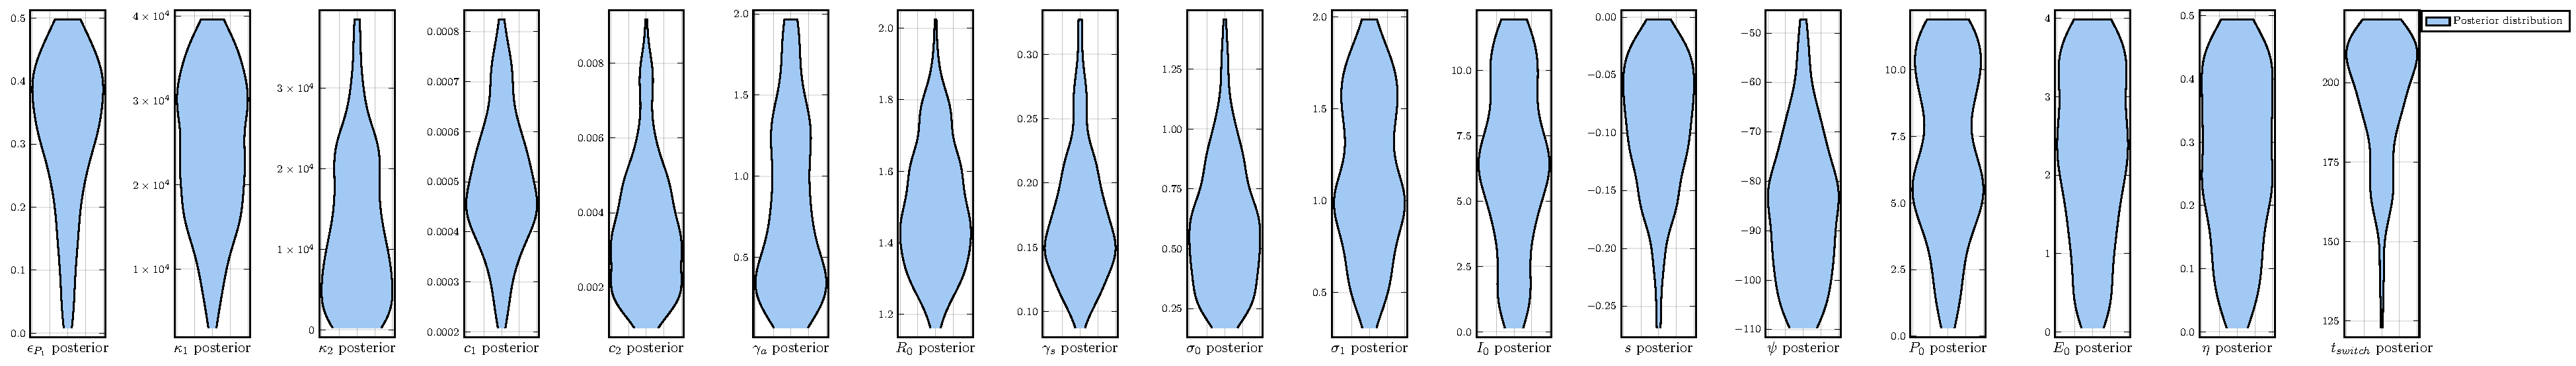
\includegraphics[width = 18 cm]{FigureS1.pdf}
\caption{\textbf{Posterior distributions on inferred non-age structured model parameters for baseline model}.Posteriors are composed of 200 candidate parameter sets from the particle filtering, the model was evaluated at these points for all future runs.}
\label{plot_model}
\end{figure}

\clearpage 

\begin{figure}[H]
\centering
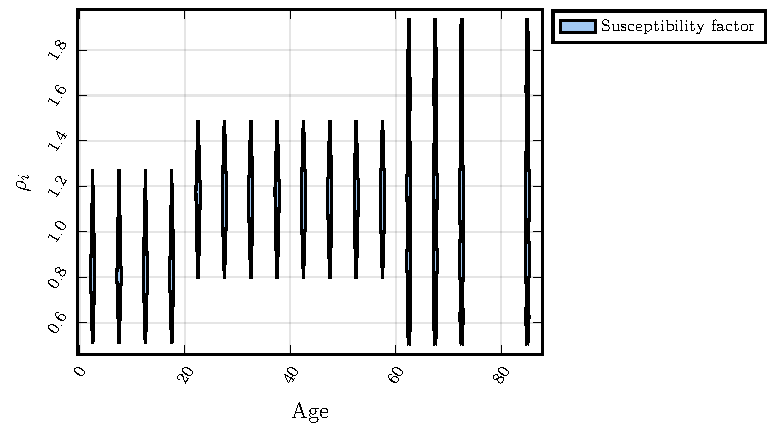
\includegraphics[width = 12 cm]{FigureS2.pdf}
\caption{\textbf{Posterior distributions on inferred age-specific susceptibility modifier parameter $\rho_i$ for baseline model}. Three age-specific susceptibility parameters shown here, $\rho_1,\rho_2,\rho_3$, were also inferred from particle filtering on the case and mobility data, corresponding to the age brackets 0-20, 20-60, 60+.}
\label{plot_model}
\end{figure}

\clearpage 

\begin{figure}[H]
\centering
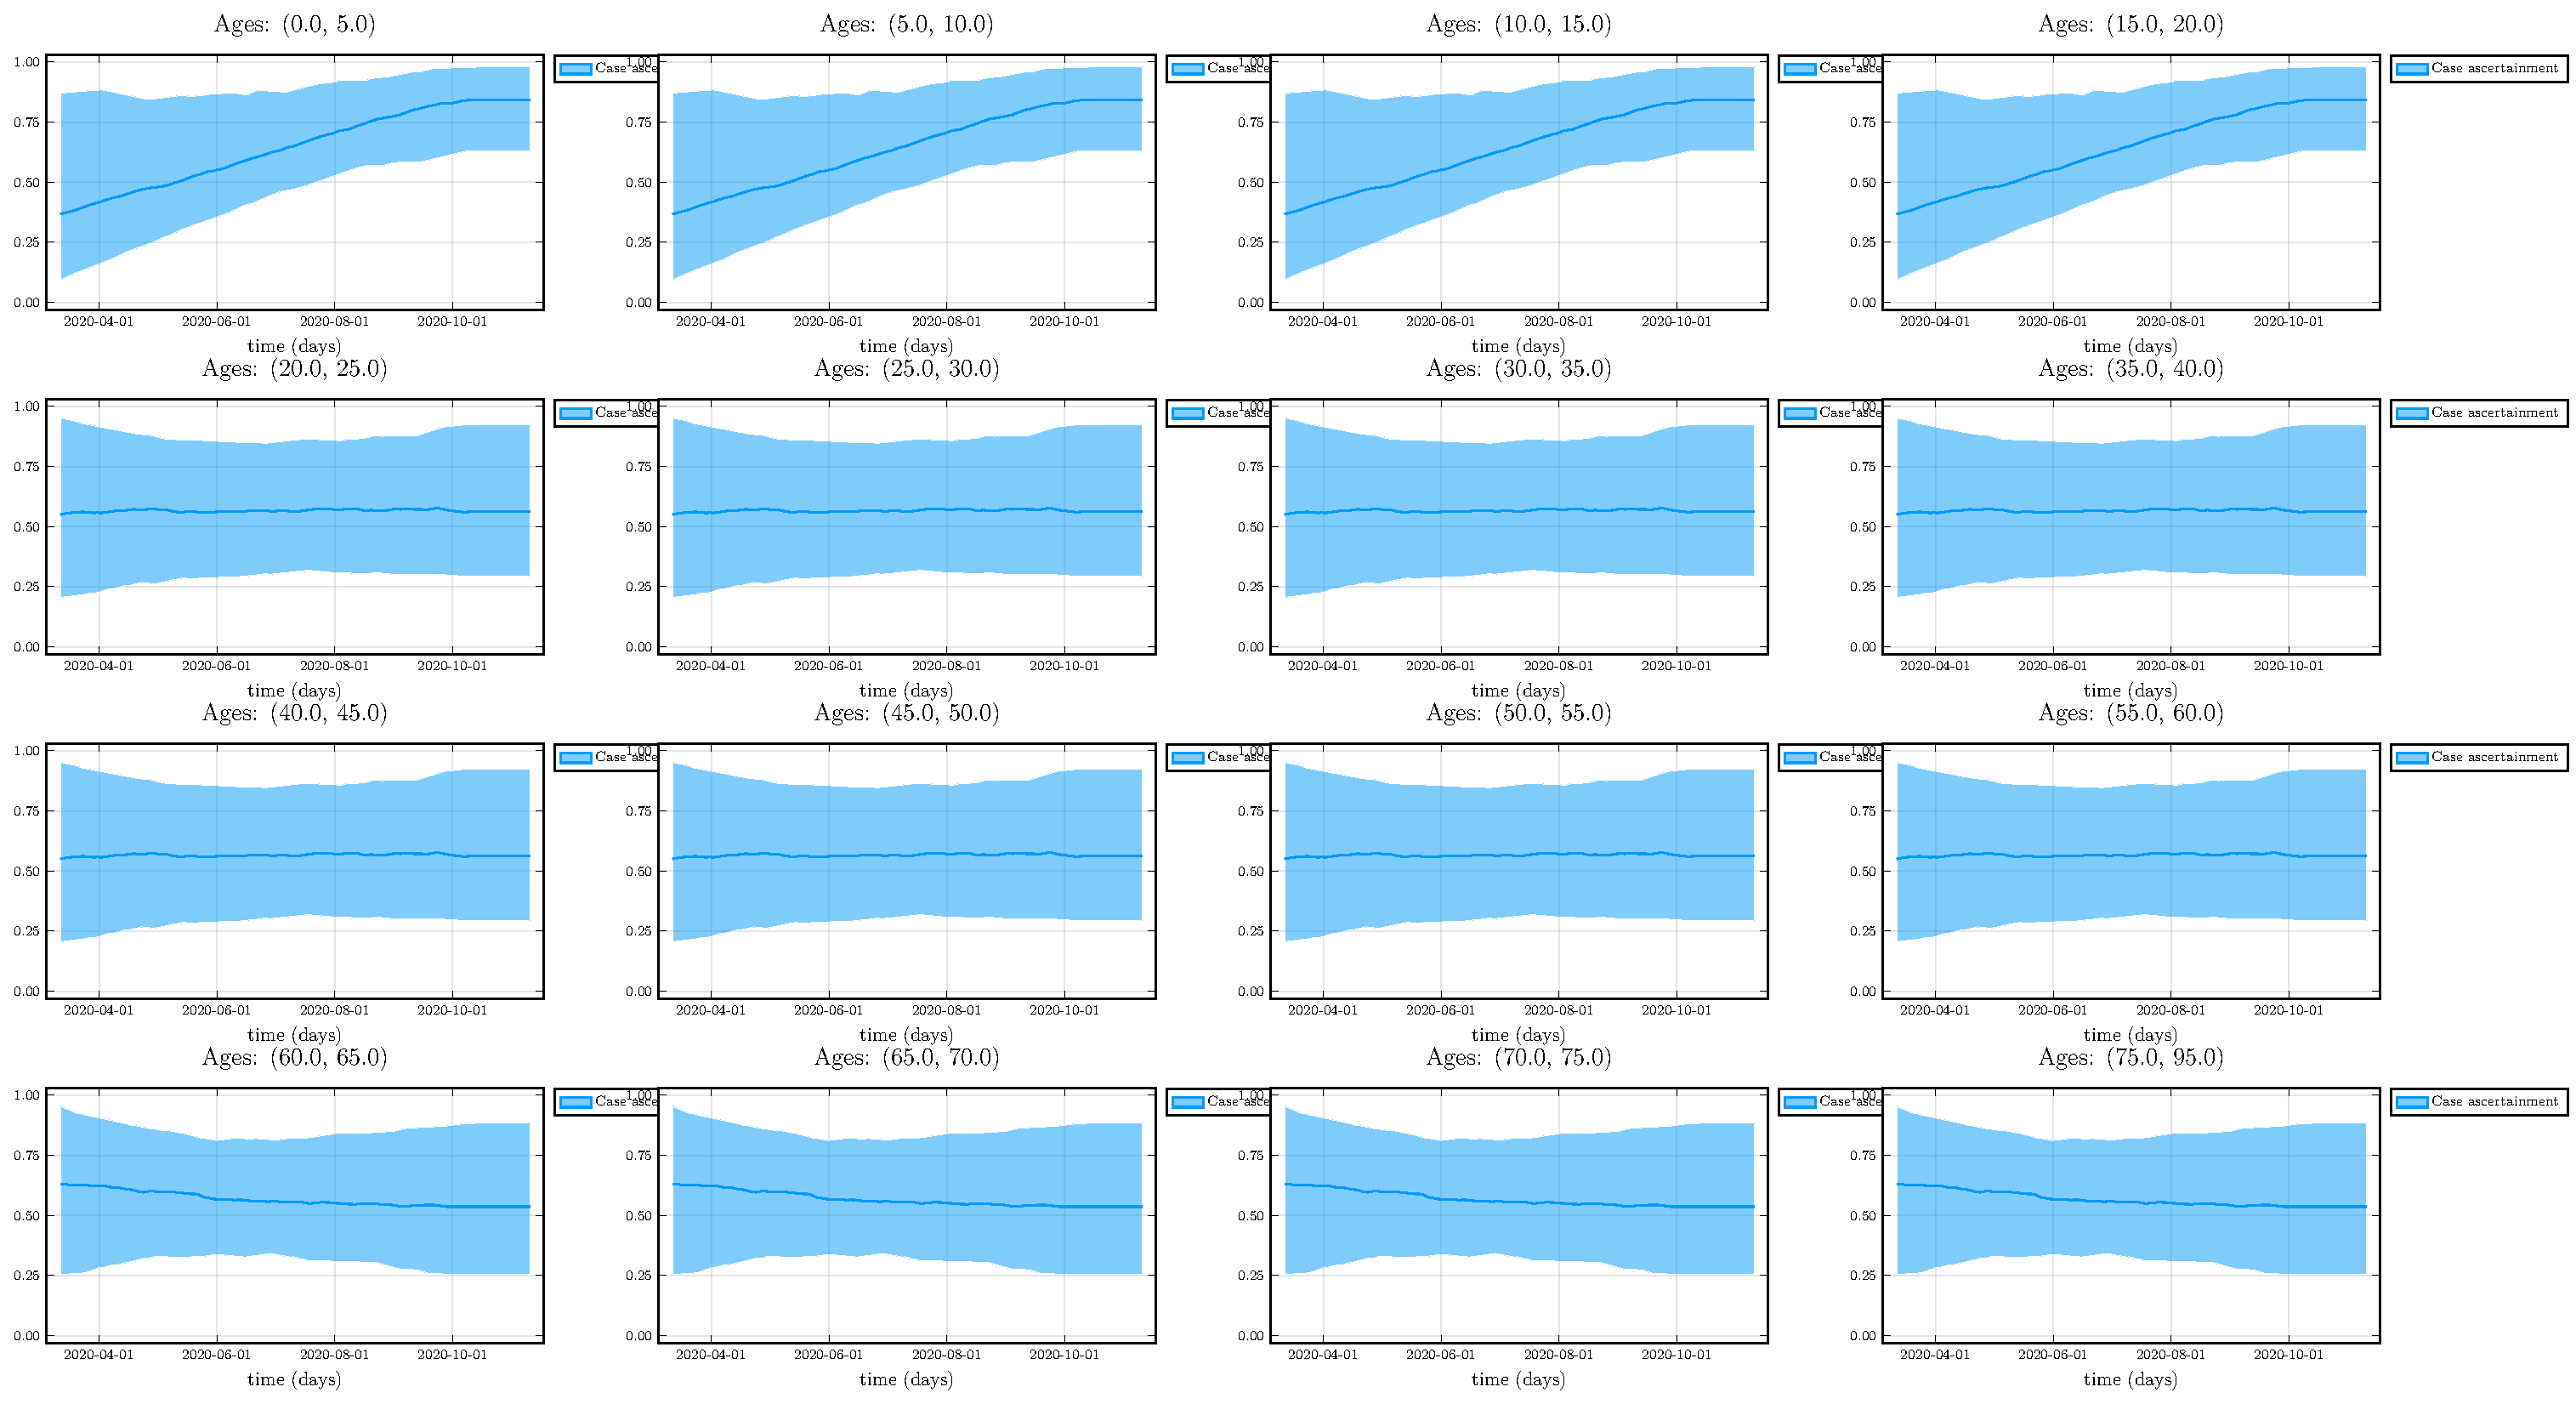
\includegraphics[width = 18 cm]{FigureS3.pdf}
\caption{\textbf{Posterior distributions on inferred age-specific ascertainment rate over time for baseline model}. Time dependent ascertainment rates inferred from the data, corresponding to the fraction of actual cases detected by the Ontario testing system. }
\label{plot_model}
\end{figure}

\clearpage 

\begin{figure}[H]
\centering
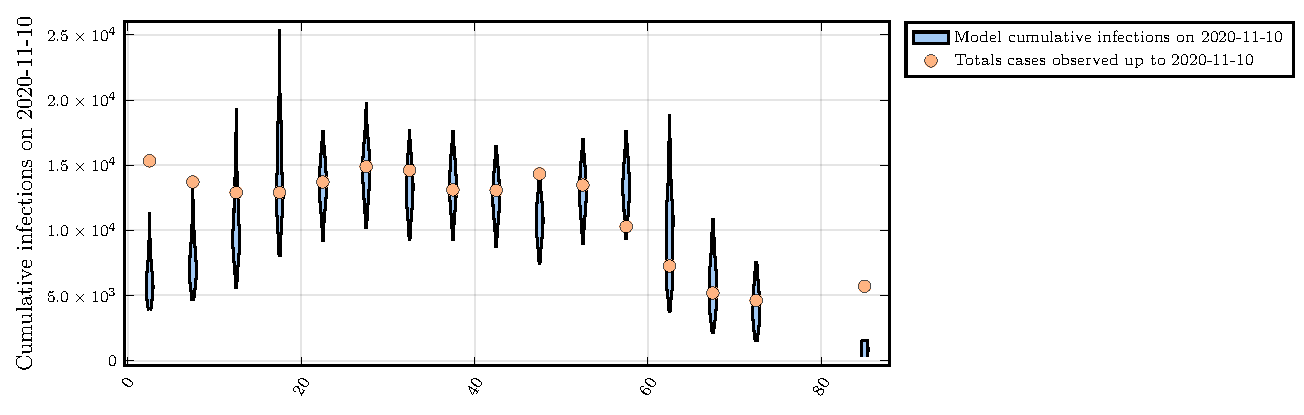
\includegraphics[width = 12 cm]{FigureS4.pdf}
\caption{\textbf{Empirical data of cumulative infections due to COVID-19 by age and model posterior predictions.} The age-specific total cases at the end of the fitting window, were used to calibrate the model, in an age dependent way. We used only three parameters to capture age specific effects and therefore trade-off some accuracy in the youngest and oldest age groups.}
\label{plot_model}
\end{figure}

\clearpage 

\begin{figure}[H]
\centering
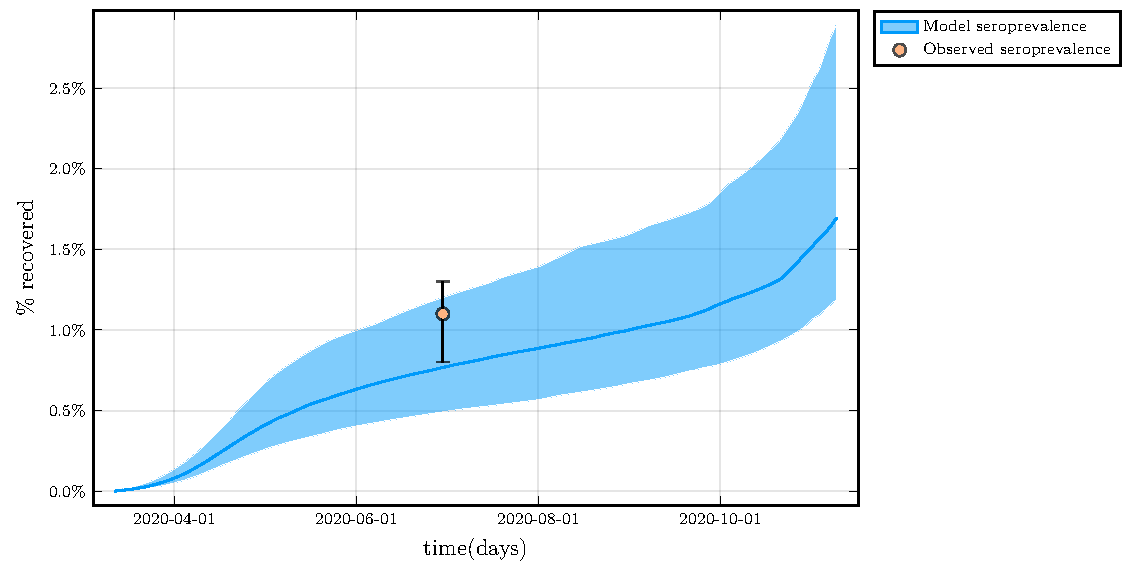
\includegraphics[width = 12 cm]{FigureS5.pdf}
\caption{\textbf{Average of model posterior population seropositivity over time, compared to empirical data.} Total seroprevalence in Ontario was assessed during the month of June. We used this value to calibrate the model further.  }
\label{plot_model}
\end{figure}

\clearpage 

\begin{figure}[H]
\centering
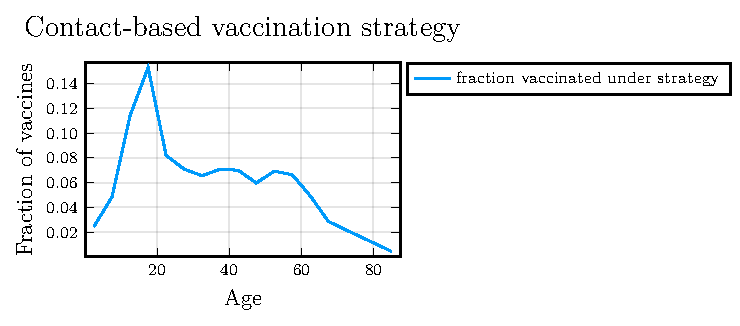
\includegraphics[width = 12 cm]{FigureS6.pdf}
\caption{\textbf{Age distribution of vaccination under the contact-based strategy.} This strategy vaccinates proportionally to the leading eigenvector of the full contact matrix, $C(0)$, to vaccinate people who will, approximately, produce the most secondary infections in a linearized regime.}
\label{plot_model}
\end{figure}

\clearpage 

\begin{figure}[H]
\centering
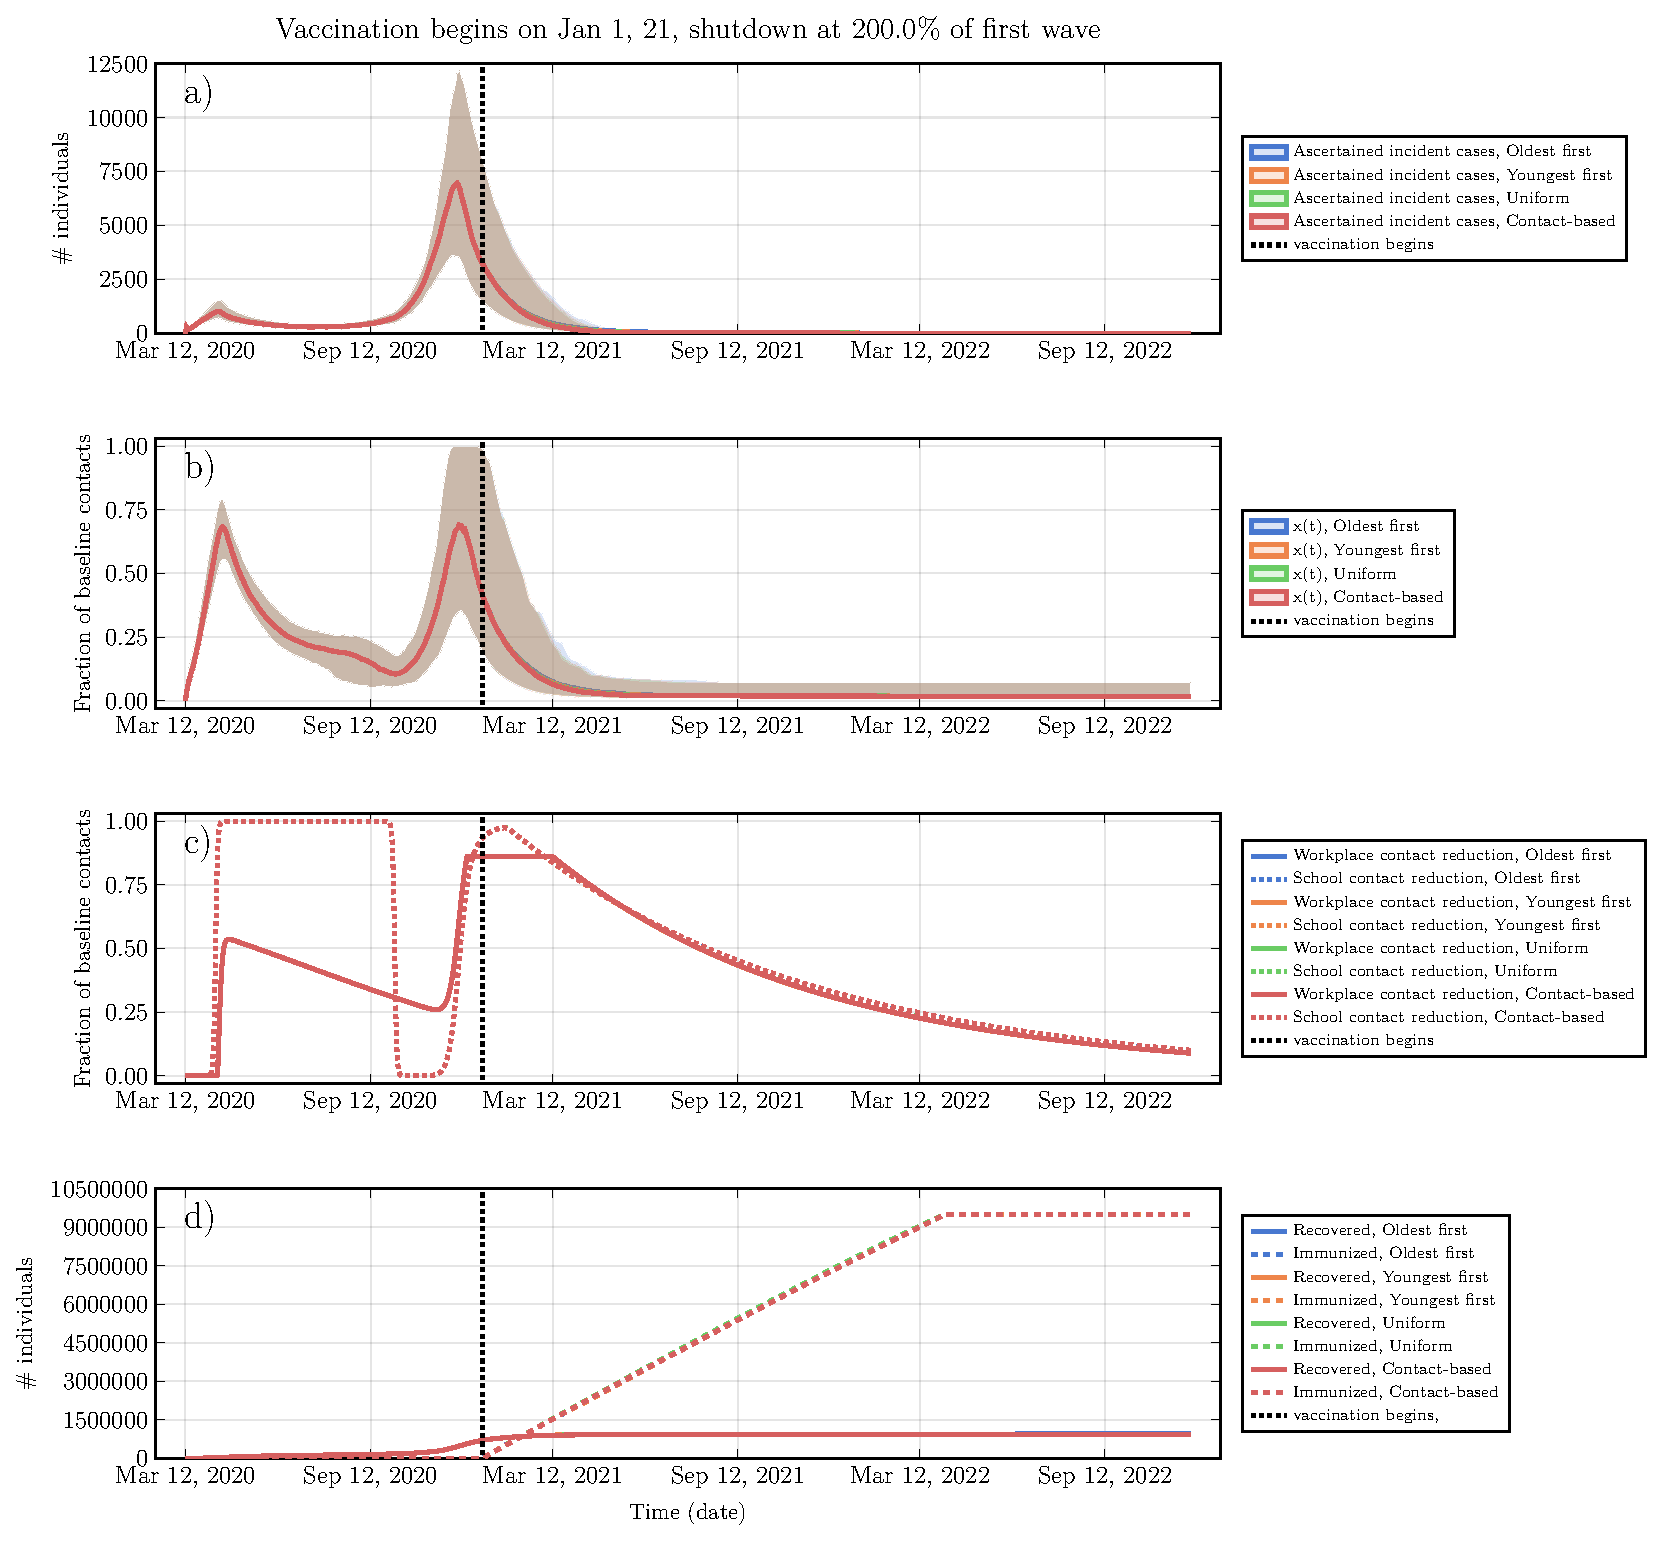
\includegraphics[width = 16 cm]{FigureS7.pdf}
\caption{\textbf{Social and epidemic dynamics for early vaccine availability and high vaccination rate.} (a) Ascertained incident COVID-19 cases, (b) proportion $x$ of the population practicing NPIs, (c) Intensity of school and workplace closure, (d) percentage of population with natural or vaccine-derived immunity versus time. $T=200 \%$, $\psi_0=1.5 \%$ per week, vaccine available in January 2021.   Other parameters are in Table \ref{tab:params}.}
\label{plot_model}
\end{figure}

\clearpage 

\begin{figure}[H]
\centering
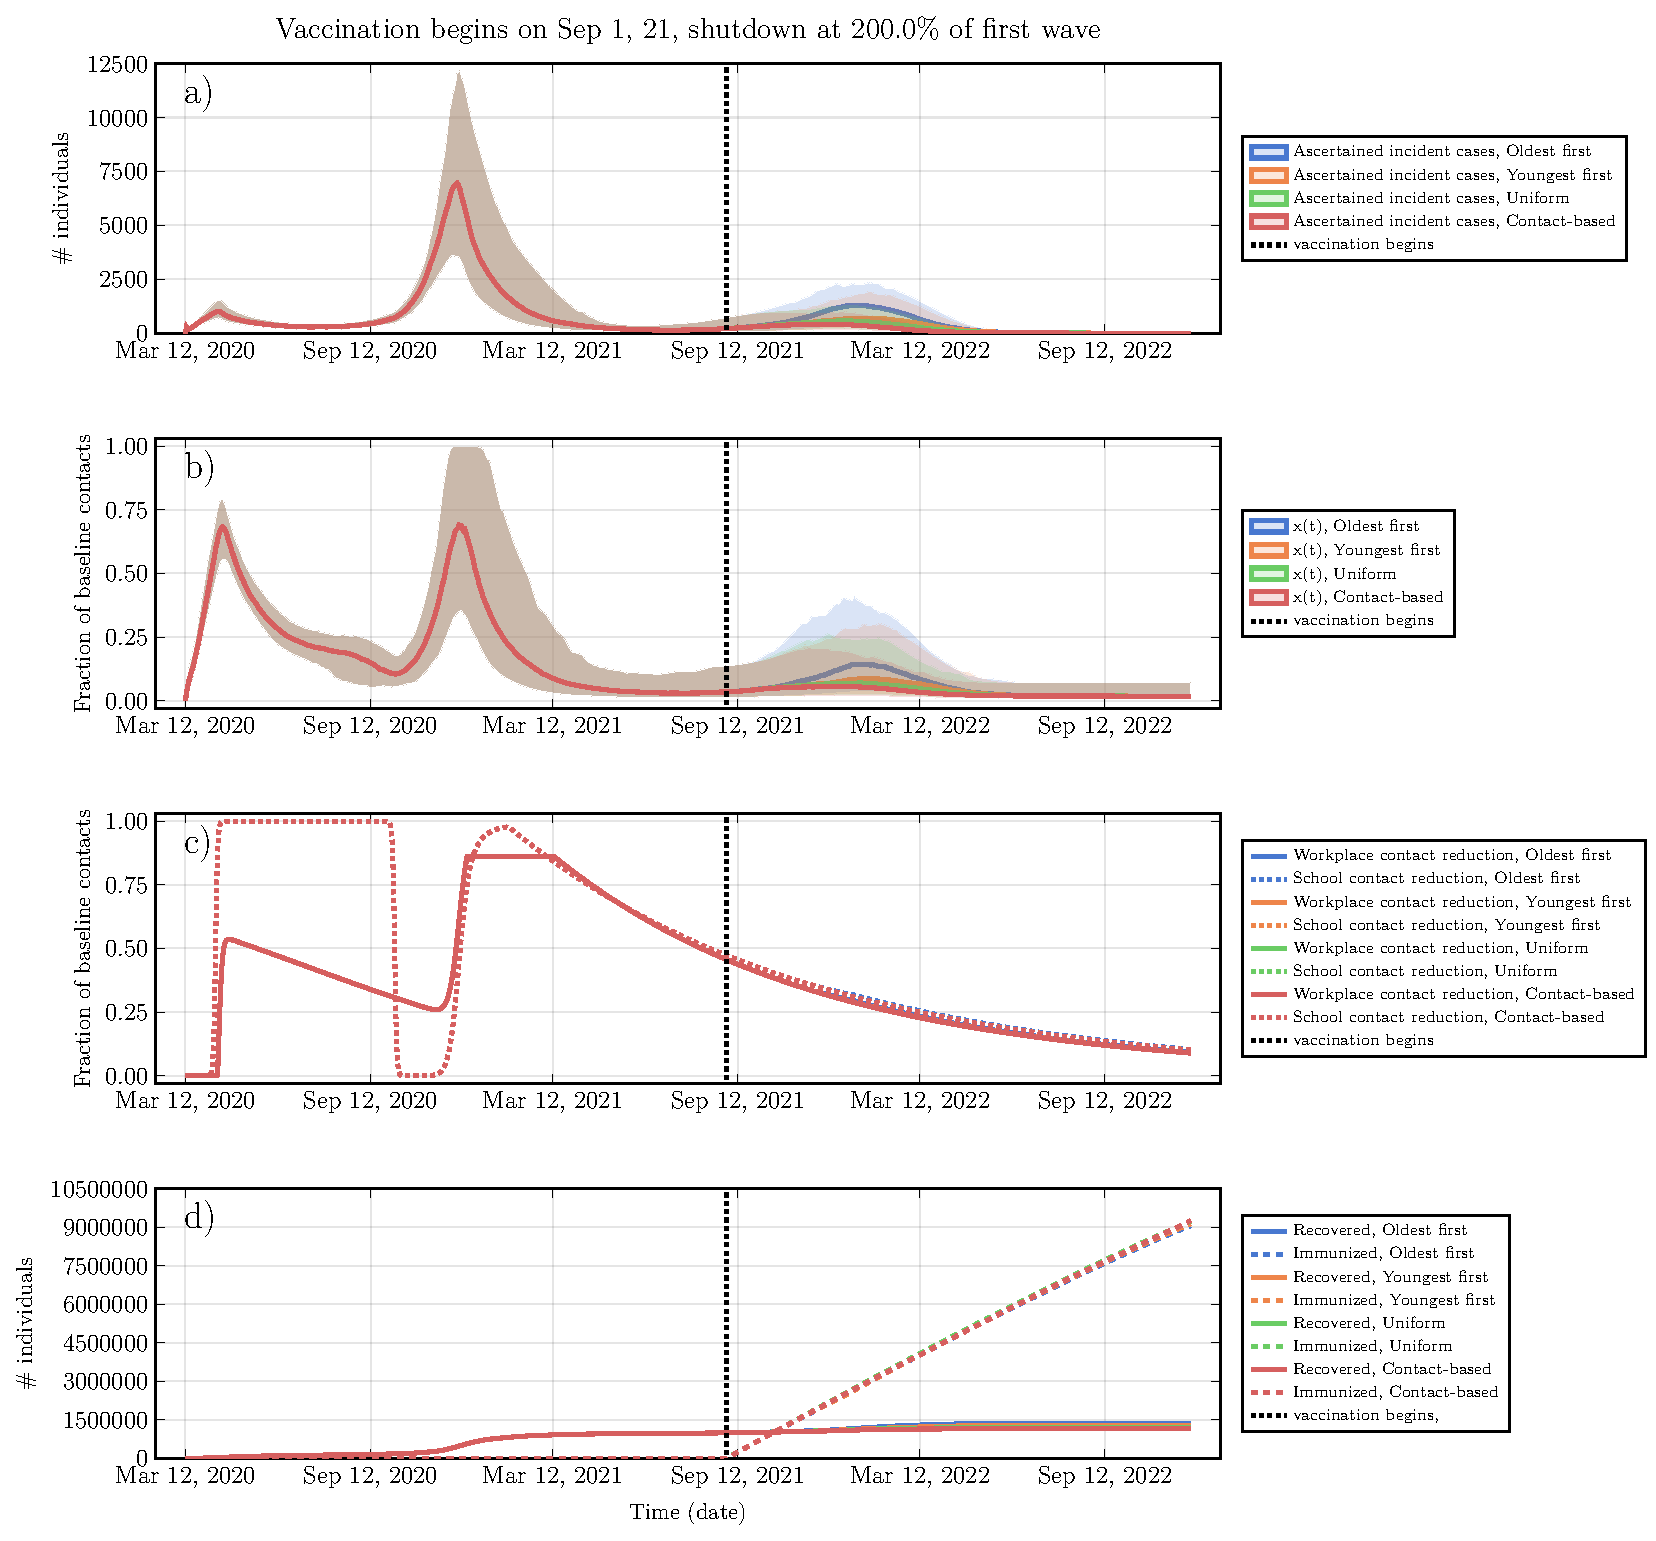
\includegraphics[width = 16 cm]{FigureS8.pdf}
\caption{\textbf{Social and epidemic dynamics for late vaccine availability and high vaccination rate.} (a) Ascertained incident  COVID-19 cases, (b) proportion $x$ of the population practicing NPIs, (c) Intensity of school and workplace closure, (d) percentage of population with natural or vaccine-derived immunity versus time. $T=200 \%$, $\psi_0=1.5 \%$ per week, vaccine available in September 2021.   Other parameters are in Table \ref{tab:params}.}
\label{plot_model}
\end{figure}

\clearpage 

\begin{figure}[H]
\centering
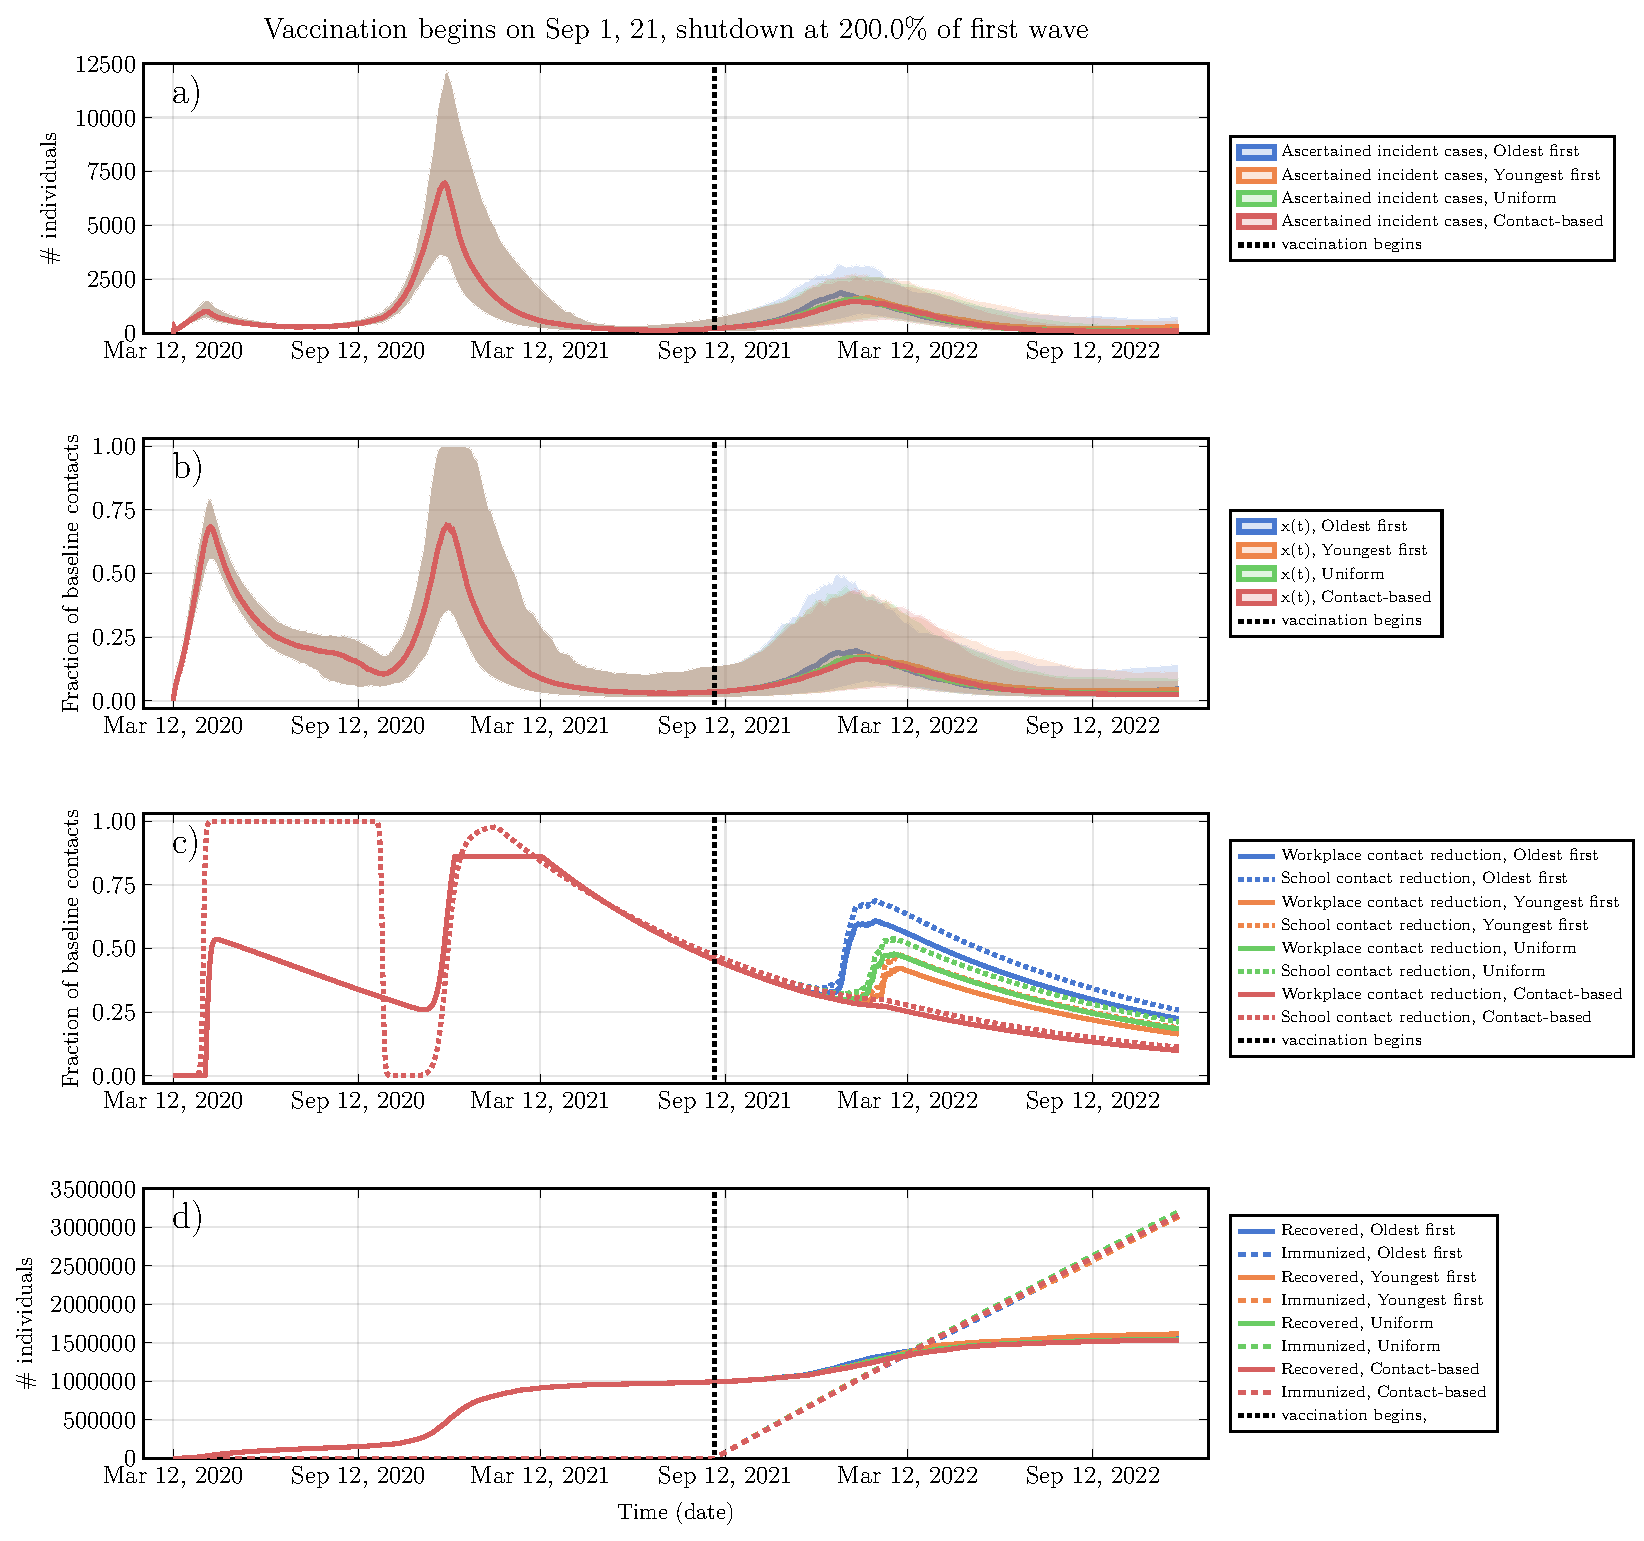
\includegraphics[width = 16 cm]{FigureS9.pdf}
\caption{\textbf{Social and epidemic dynamics for late vaccine availability and low vaccination rate.} (a) Ascertained incident COVID-19 cases, (b) proportion $x$ of the population practicing NPIs, (c) Intensity of school and workplace closure, (d) percentage of population with natural or vaccine-derived immunity versus time. $T=200 \%$, $\psi_0=0.5 \%$ per week, vaccine available in September 2021.   Other parameters are in Table \ref{tab:params}.}
\label{plot_model}
\end{figure}


\clearpage 

\begin{figure}[H]
\centering
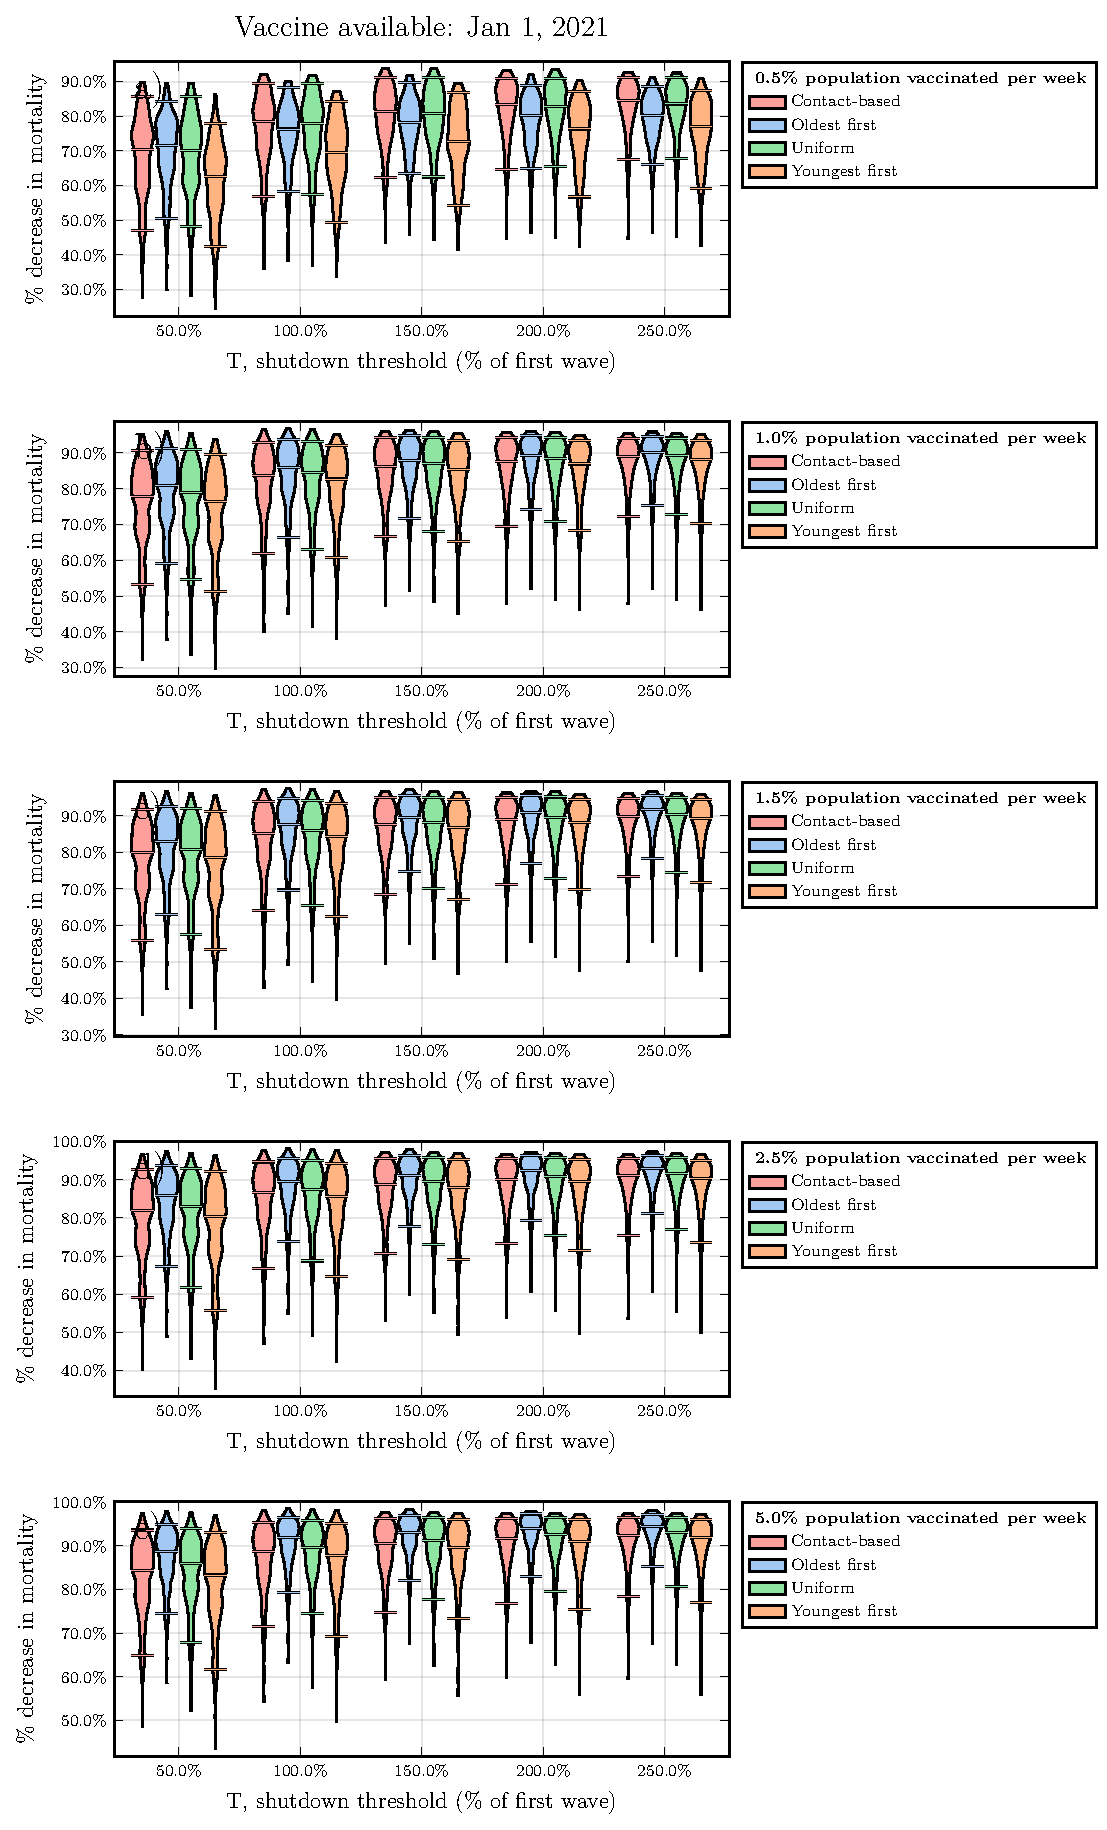
\includegraphics[width = 12 cm]{FigureS10.pdf}
\caption{\textbf{Mortality reductions under various values of $T$ and $\psi_0$, early vaccine availability.} Violin plots of the percent reduction in mortality under the four vaccine strategies, relative to no vaccination, as a function of the vaccination rate $\psi_0$, for January 2021 availability. Horizontal lines represent median values of posterior model projections. Other parameter values in Table S1.  Percentage reductions are relative to no vaccination.  Projected number of deaths in the absence of vaccination were 35597.2 (CI: 57465.9,19507.9); 48518.8 (CI: 86853.9,28335.7), 61339.1 (CI: 106623.0,34613.5), 
72007.3 (CI: 121754.0,40483.4); 80707.6 (CI: 126732.0,47755.4) after January 1, 2021, for T=50\%, 100\%, 150\%, 200\%, and 250\%, respectively. }
\label{plot_model}
\end{figure}




\clearpage 


\begin{figure}[H]
\centering
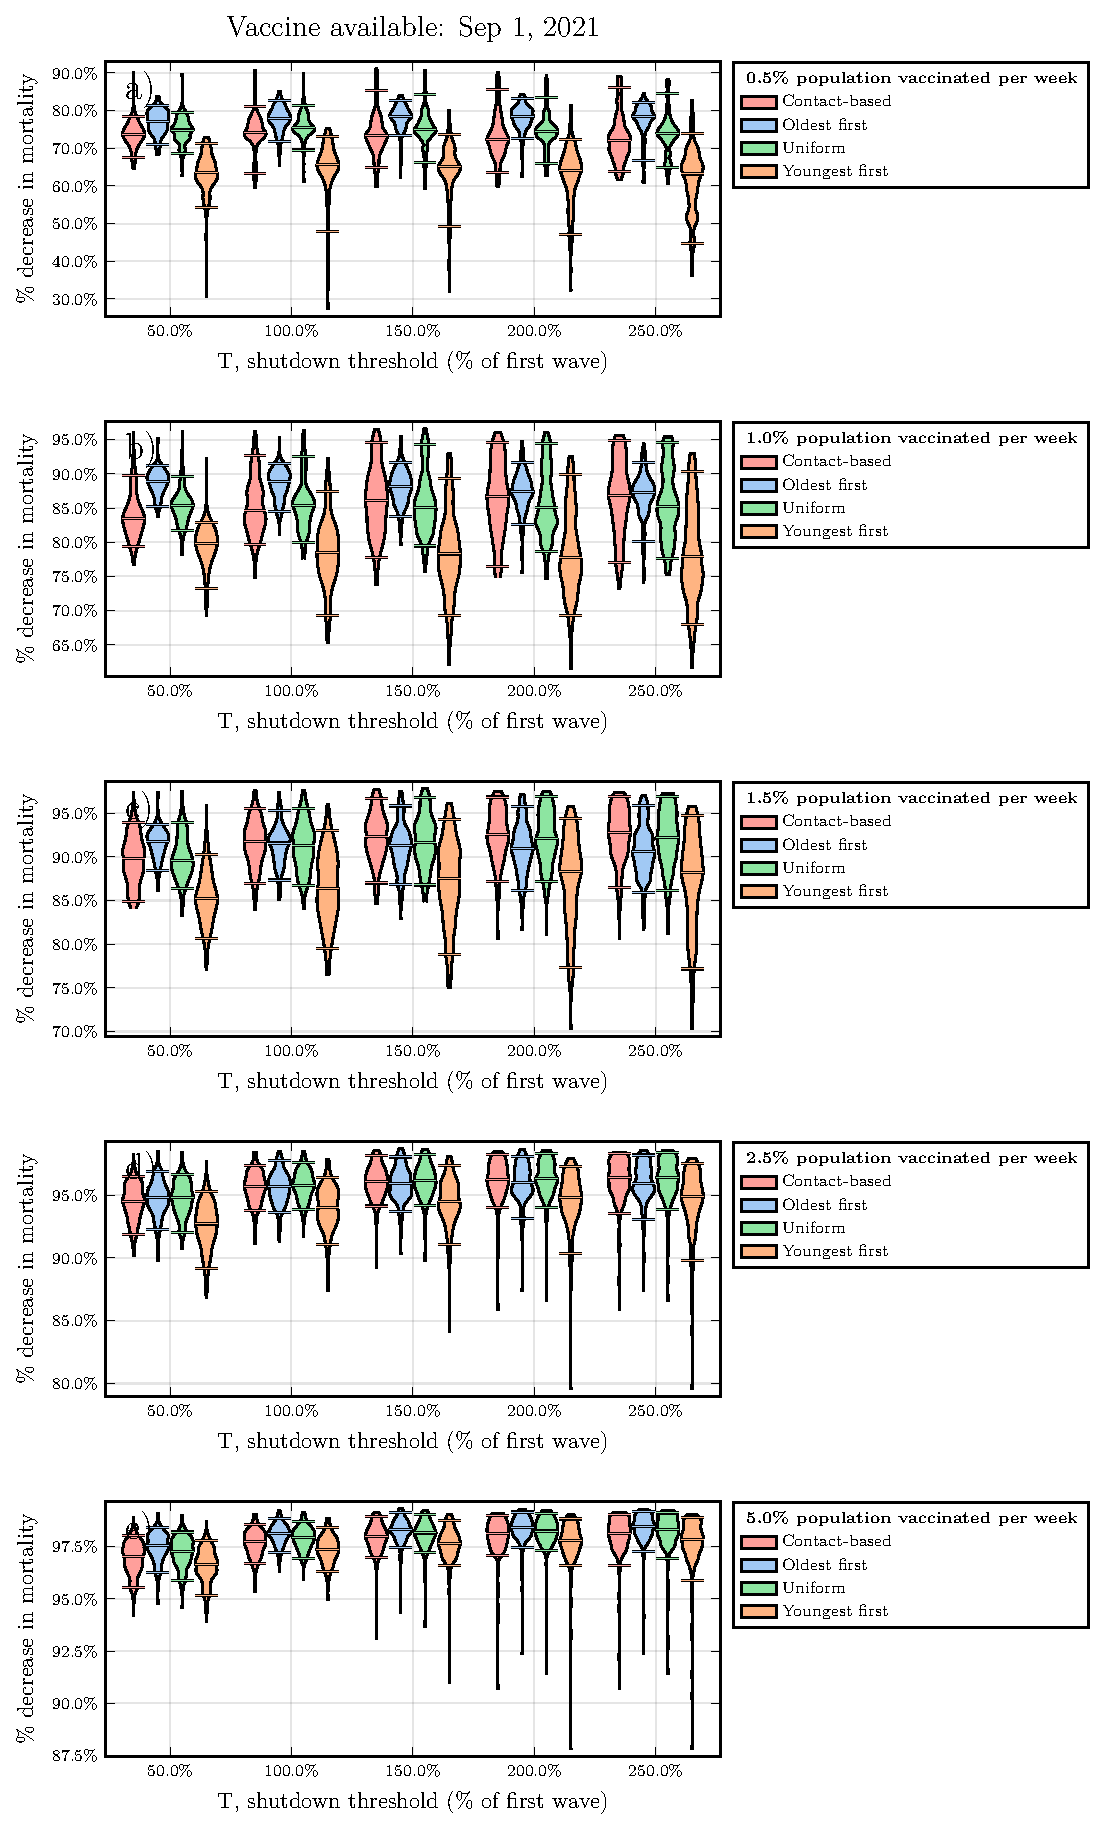
\includegraphics[width = 12 cm]{FigureS11.pdf}
\caption{\textbf{Mortality reductions under various values of $T$ and $\psi_0$, late vaccine availability.} Violin plots of the percent reduction in mortality under the four vaccine strategies, relative to no vaccination, as a function of the vaccination rate $\psi_0$, for September 2021 availability. Horizontal lines represent median values of posterior model projections. Other parameter values in Table S1.  Percentage reductions are relative to no vaccination. Projected number of deaths in the absence of vaccination were 25478.8 (CI: 45679.0,13006.7); 39149.6 (CI: 73917.1,20290.9); 50775.1 (CI: 95451.2,25980.9); 60250.7 (CI: 108361.0,30721.9); 68594.0 (CI: 107157.0,36063.6) after September 1, 2021 for T=50\%, 100\%, 150\%, 200\%, and 250\%, respectively. }
\label{plot_model}
\end{figure}



\clearpage 


\begin{figure}[H]
\centering
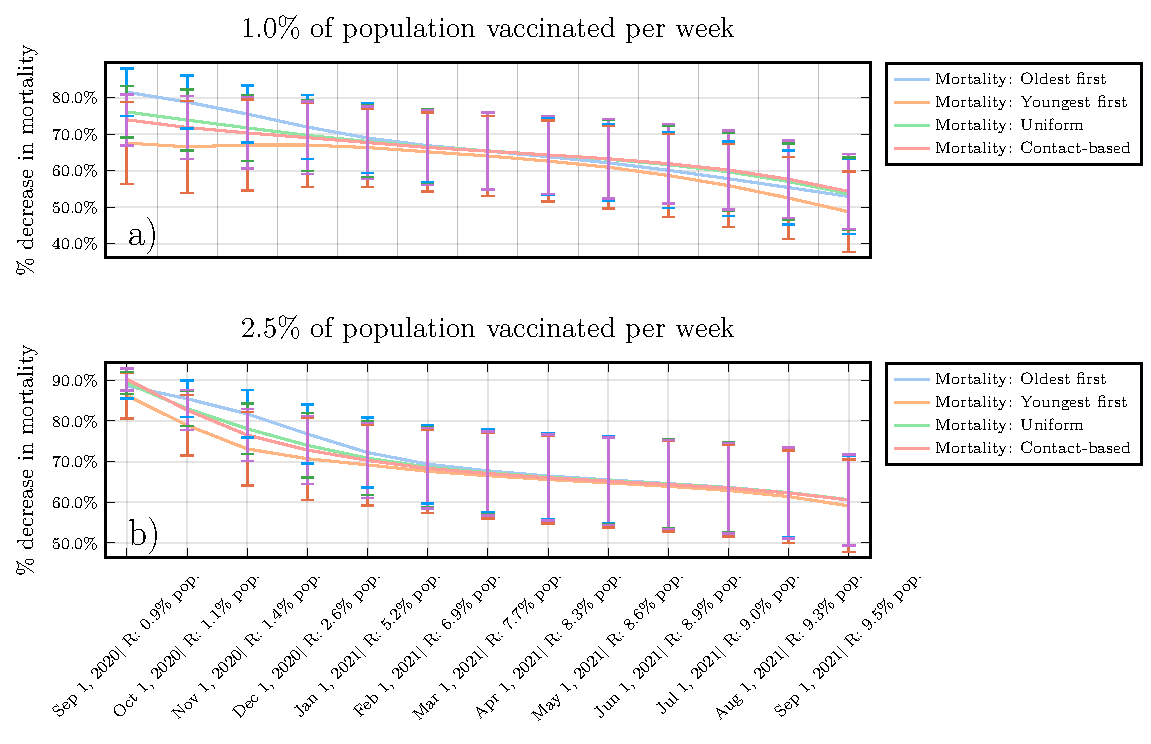
\includegraphics[width = 15 cm]{FigureS12.pdf}
\caption{\textbf{A higher level of natural immunity increases the relative advantage of transmission-interrupting strategies.}  Median and standard deviation of the percent reduction in mortality under the four vaccine strategies, relative to no vaccination, as a function of the vaccination start date and percent recovered at that time, for (a) $\phi_0=1.0 \%$ vaccinated per week and (b) $\phi_0=2.5 \%$ vaccinated per week.  Shutdown threshold $T=200 \%$,  and other parameter values in Appendix, Table S1.}
\label{plot_model}
\end{figure}

\clearpage 

\begin{figure}[H]
\centering
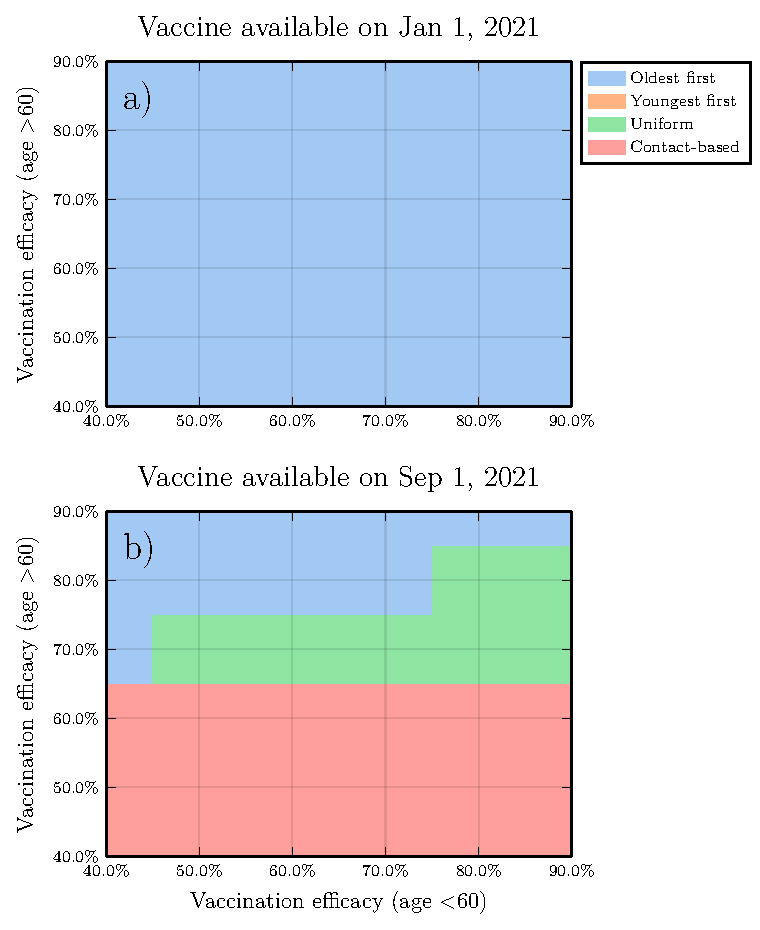
\includegraphics[width = 14 cm]{FigureS13.pdf}
\caption{\textbf{Sensitivity analysis exploring a range of vaccine efficacy values, for vaccination rate $\phi_0=2.5 \%$ per week.} Subpanels are parameter planes for January and September availability showing the vaccination strategy that reduces COVID-19 mortality the most as a function of vaccine efficacy in $60+$ year-olds versus vaccine efficacy in other age groups. Other parameter values as in Table S1.}
\label{plot_model}
\end{figure}

\clearpage 

\begin{figure}[H]
\centering
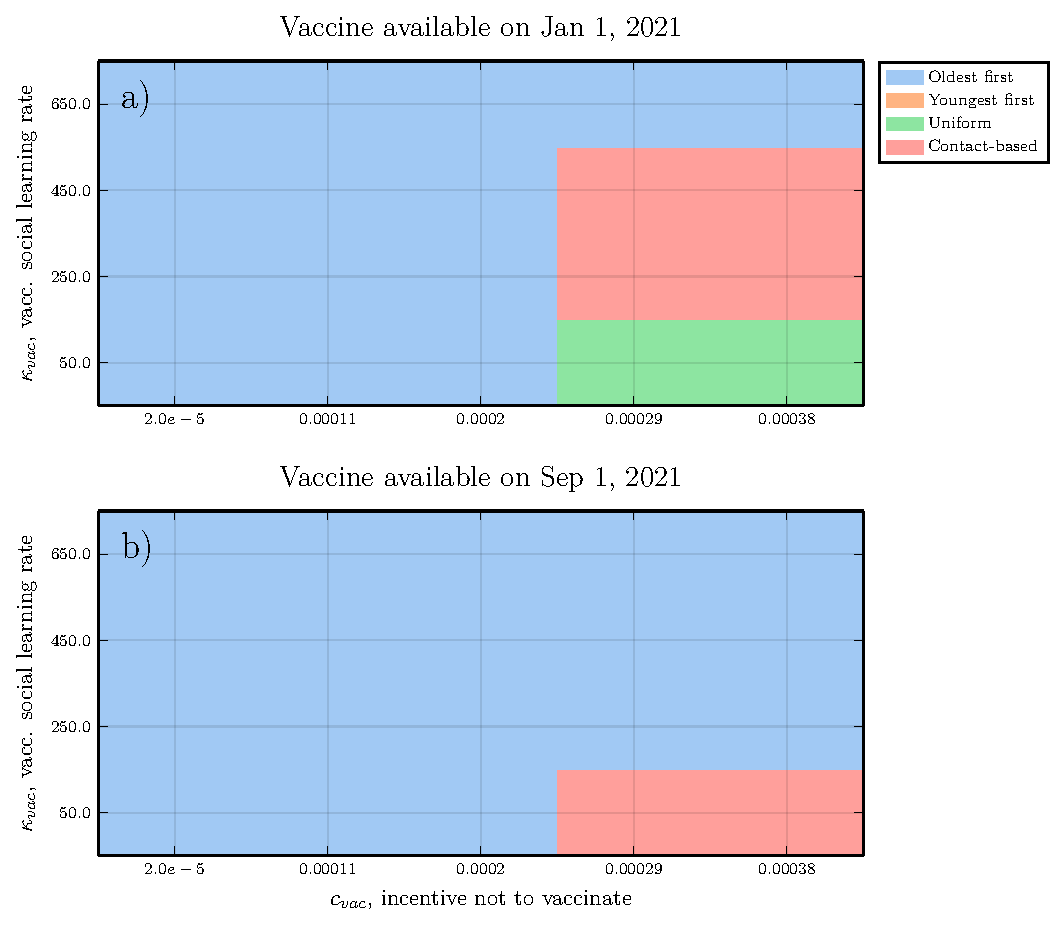
\includegraphics[width = 14 cm]{FigureS14.pdf}
\caption{\textbf{Sensitivity analysis exploring impact of vaccinating behaviour dynamics.} $\phi_0 = 2.5 \%$ per week, $T=200 \%$. Subpanels are parameter planes for January and September availability showing the vaccination strategy that reduces COVID-19 mortality the most as a function of vaccine social learning rate $\kappa_{vac}$ and vaccine cost parameter $c_{vac}$. Other parameter values as in Table S1.}
\label{plot_model}
\end{figure}

\clearpage 

\begin{figure}[H]
\centering
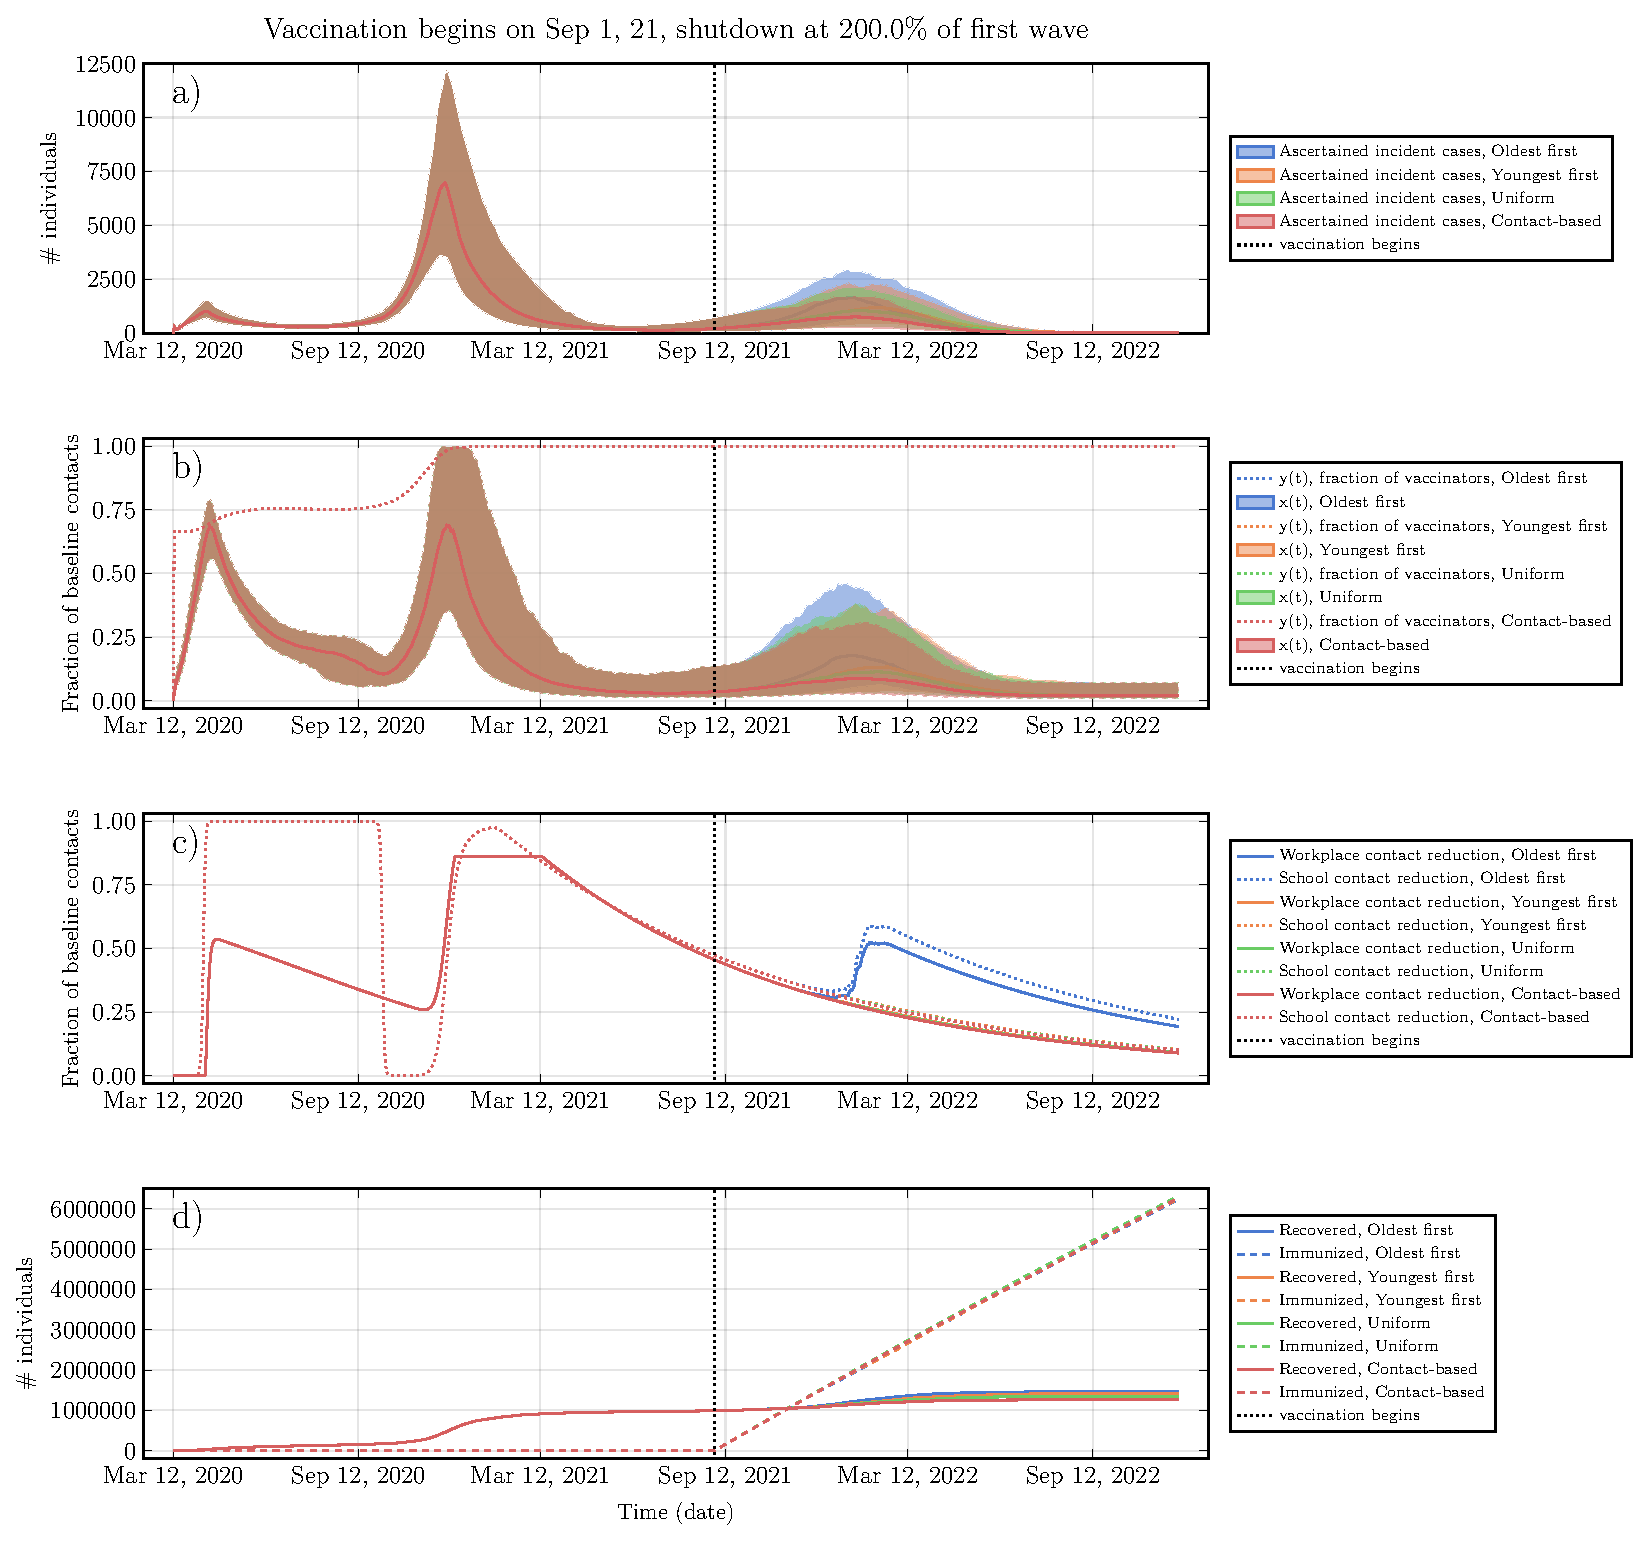
\includegraphics[width = 16 cm]{FigureS15.pdf}
\caption{\textbf{Epidemic dynamics and social dynamics for both NPI adherence and vaccinating behaviour, when vaccine cost is small, $c_{vac}=1.1\times 10^{-4}$.} (a) Ascertained incident COVID-19 cases, (b) proportion $x$ of the population practicing NPIs, (c) Intensity of school and workplace closure, (d) percentage of population with natural or vaccine-derived immunity versus time. $T=200 \%$, $\psi_0=1.0 \%$ per week (maximum rate in absence of vaccine refusal), vaccine available in September 2021, $\kappa_{vac}=50$/day.   Other parameters are in Table \ref{tab:params}.}
\label{plot_model}
\end{figure}

\clearpage 

\begin{figure}[H]
\centering
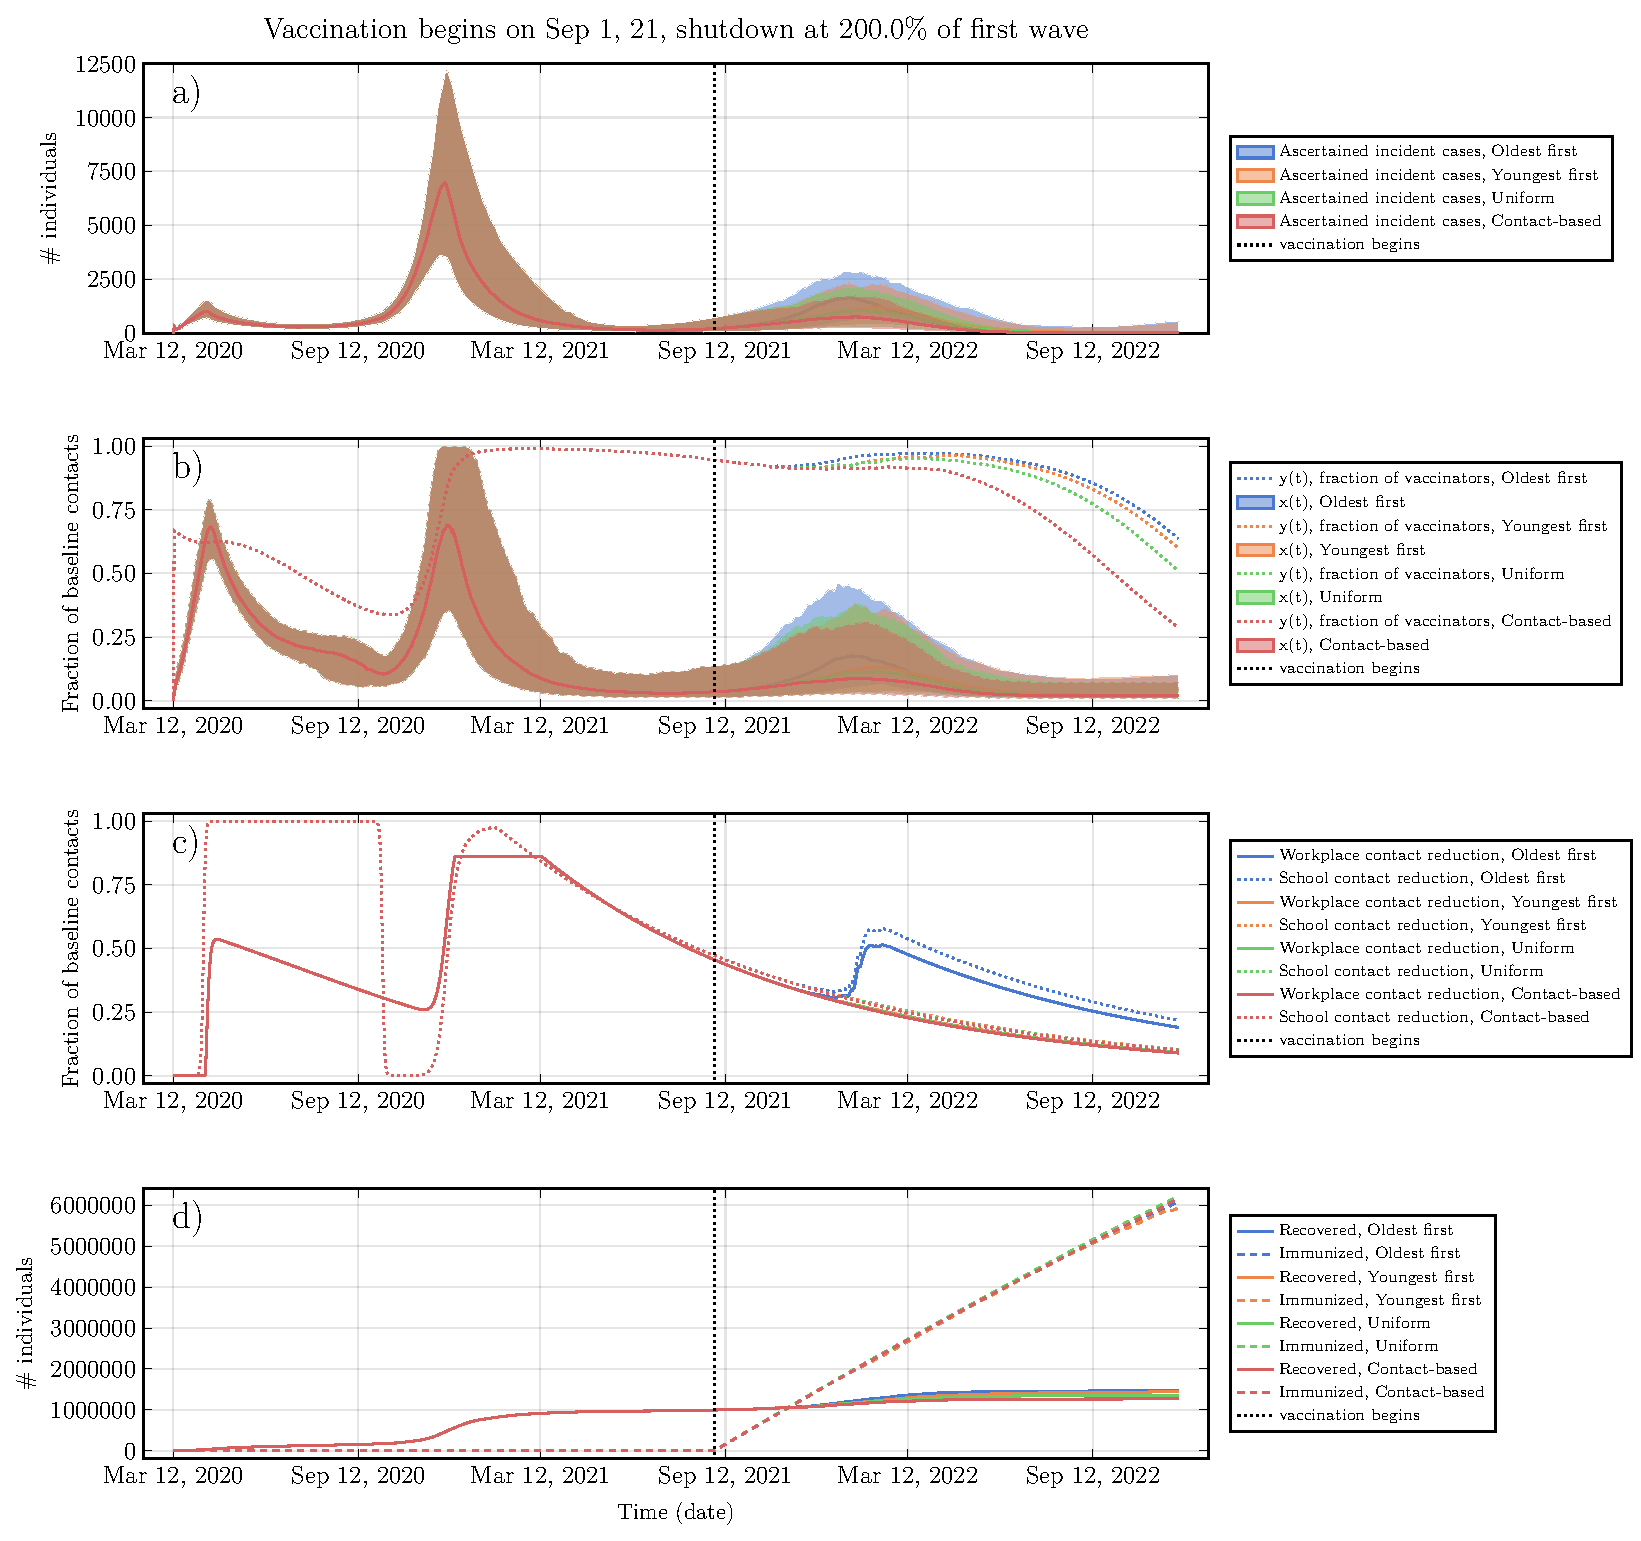
\includegraphics[width = 16 cm]{FigureS16.pdf}
\caption{\textbf{Epidemic dynamics and social dynamics for both NPI adherence and vaccinating behaviour, when vaccine cost is moderate, $c_{vac}=2.9\times 10^{-4}$.} (a) Ascertained incident COVID-19 cases, (b) proportion $x$ of the population practicing NPIs, (c) Intensity of school and workplace closure, (d) percentage of population with natural or vaccine-derived immunity versus time. $T=200 \%$, $\psi_0=1.0 \%$ per week (maximum rate in absence of vaccine refusal), vaccine available in September 2021, $\kappa_{vac}=50$/day.   Other parameters are in Table \ref{tab:params}.}
\label{plot_model}
\end{figure}

\clearpage 

\begin{figure}[H]
\centering
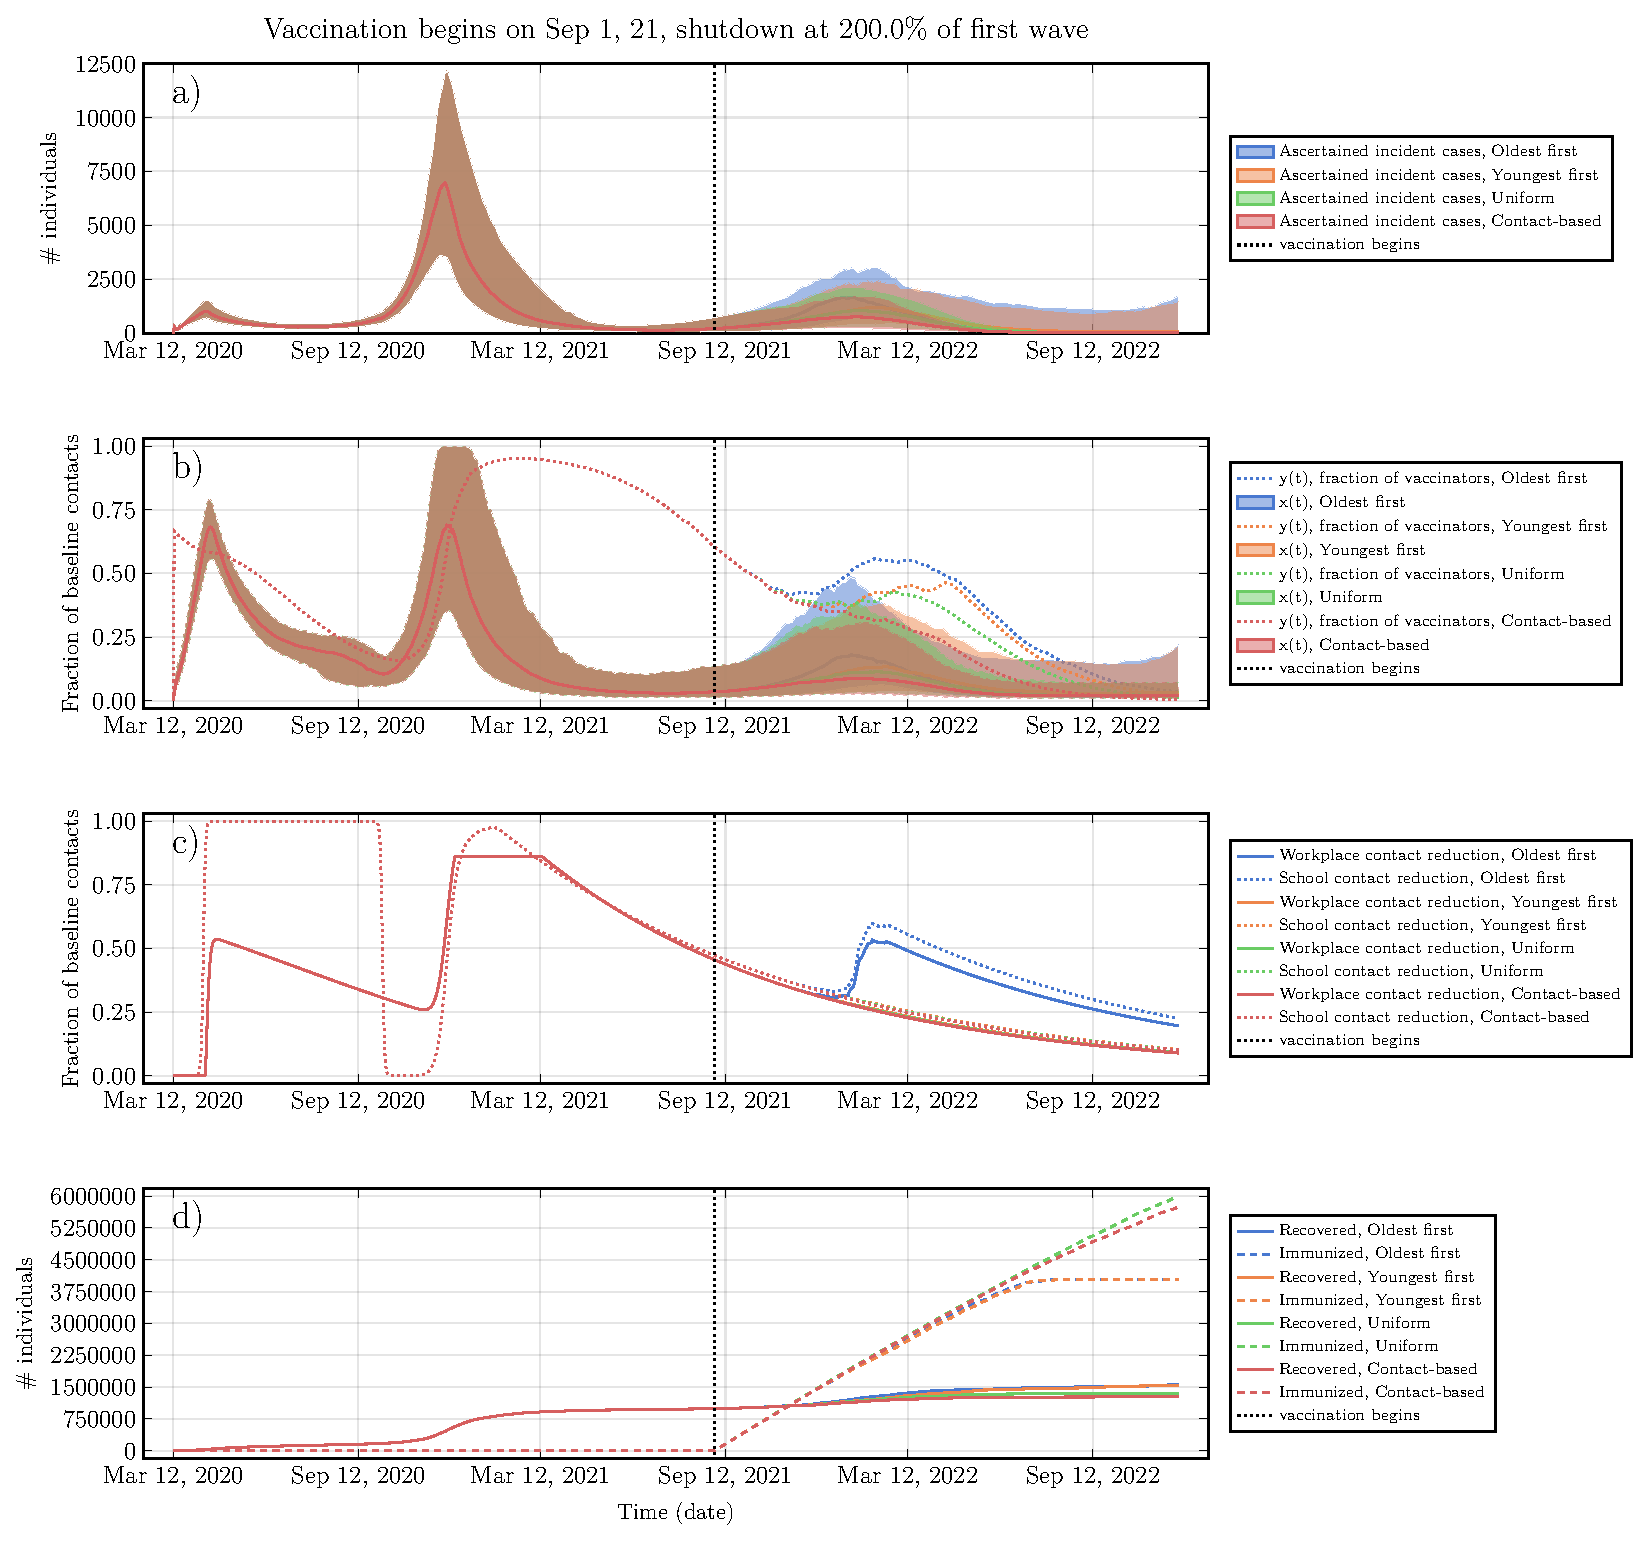
\includegraphics[width = 16 cm]{FigureS17.pdf}
\caption{\textbf{Epidemic dynamics and social dynamics for both NPI adherence and vaccinating behaviour, when vaccine cost is high, $c_{vac}=3.8\times 10^{-4}$.} (a) Ascertained incident COVID-19 cases, (b) proportion $x$ of the population practicing NPIs, (c) Intensity of school and workplace closure, (d) percentage of population with natural or vaccine-derived immunity versus time. $T=200 \%$, $\psi_0=1.0 \%$ per week (maximum rate in absence of vaccine refusal), vaccine available in September 2021, $\kappa_{vac}=50$/day. Other parameters are in Table \ref{tab:params}.}
\label{plot_model}
\end{figure}

\clearpage 

\begin{figure}[H]
\centering
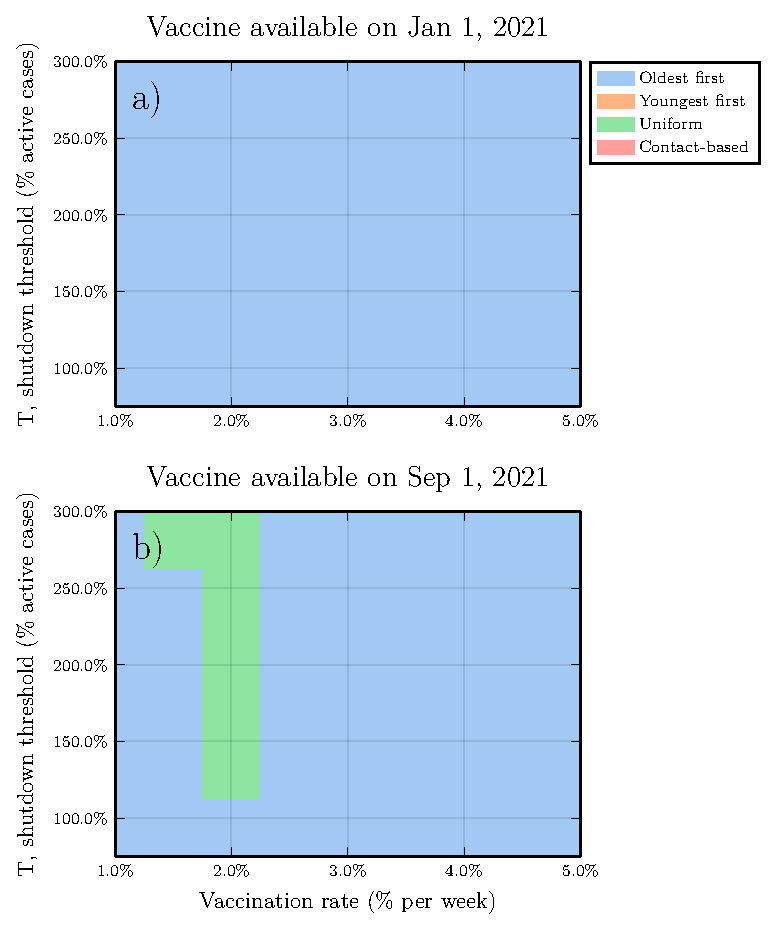
\includegraphics[width = 14 cm]{FigureS18.pdf}
\caption{\textbf{Sensitivity analysis for the scenario where $R_0=2.5$ for December 2020 onward.} Subpanels are (left) parameter planes for January and September availability showing the vaccination strategy that prevents the most COVID-19 deaths as a function of $T$ and $\psi_0$, and (right) percentage reductions in mortality. Other parameter values are as in Table S1.}
\label{plot_model}
\end{figure}

\clearpage 

\begin{figure}[H]
\centering
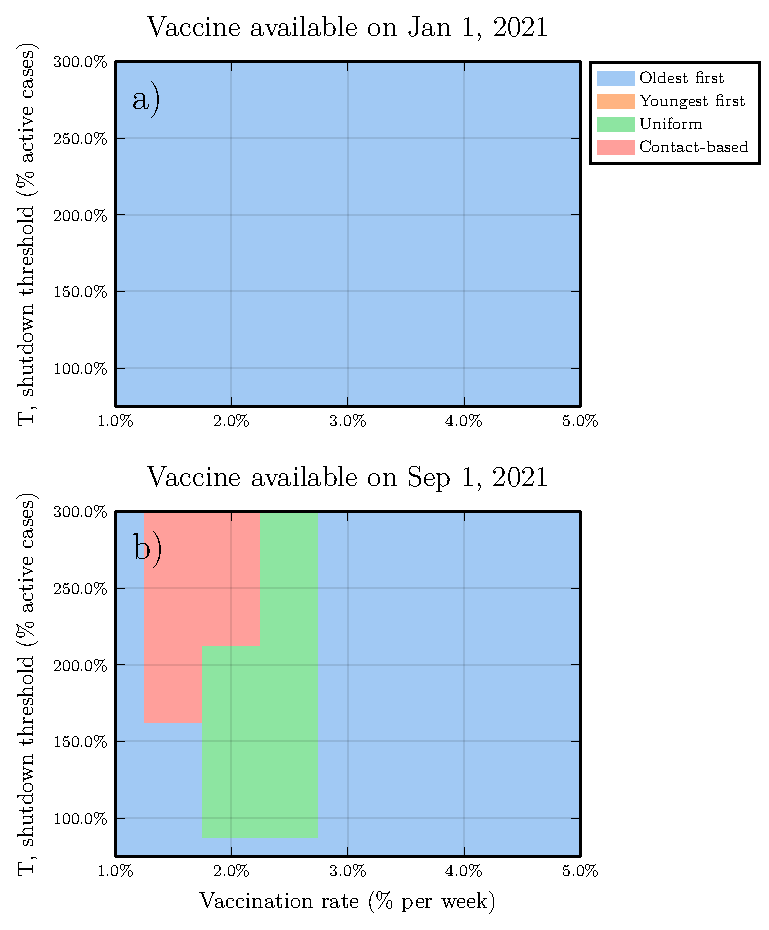
\includegraphics[width = 14 cm]{FigureS19.pdf}
\caption{\textbf{Sensitivity analysis for the scenario of $30 \%$ heightened ascertainment across all ages from December 2020 onward.} Subpanels are parameter planes for January and September availability showing the vaccination strategy that reduces COVID-19 mortality the most as a function of $T$ and $\psi_0$ (left) and the corresponding posterior parameter distributions for the refitted parameters (right).  Other parameter values as in Table S1.}
\label{plot_model}
\end{figure}

\clearpage 

\begin{figure}[H]
\centering
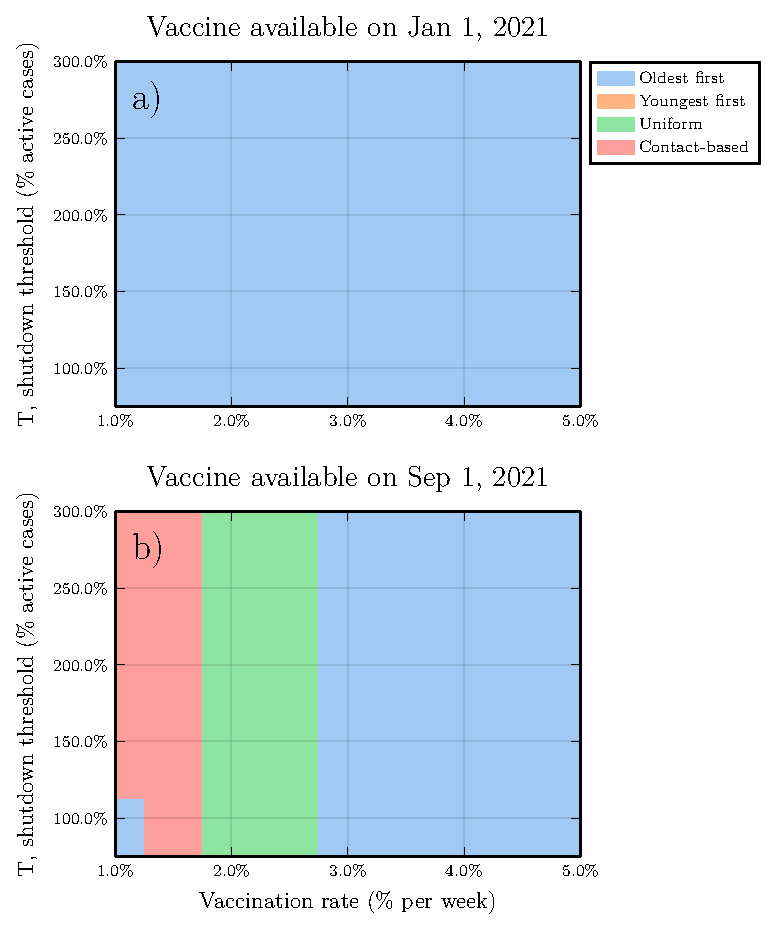
\includegraphics[width = 14 cm]{FigureS20.pdf}
\caption{\textbf{Sensitivity analysis for the scenario of $30 \%$ reduced ascertainment across all ages from December 2020 onward.} Subpanels are parameter planes for January and September availability showing the vaccination strategy that reduces COVID-19 mortality the most as a function of $T$ and $\psi_0$ (left) and the corresponding posterior parameter distributions for the refitted parameters (right).  Other parameter values as in Table S1.}
\label{plot_model}
\end{figure}

\clearpage 


\begin{figure}[H]
\centering
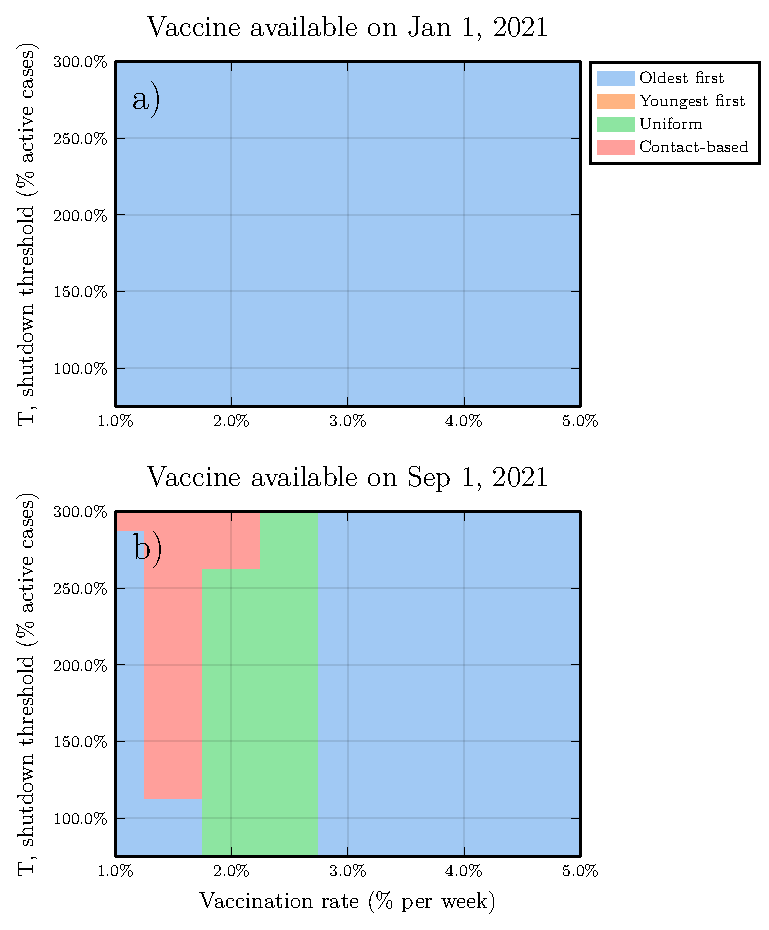
\includegraphics[width = 14 cm]{FigureS21.pdf}
\caption{\textbf{Sensitivity analysis for the scenario of four times the baseline social learning rate from December 2020 onward.} Subpanels are parameter planes for January and September availability showing the vaccination strategy that reduces COVID-19 mortality the most as a function of $T$ and $\psi_0$ (left) and the corresponding posterior parameter distributions for the refitted parameters (right).  Other parameter values as in Table S1.}
\label{plot_model}
\end{figure}

\clearpage 

\begin{figure}[H]
\centering
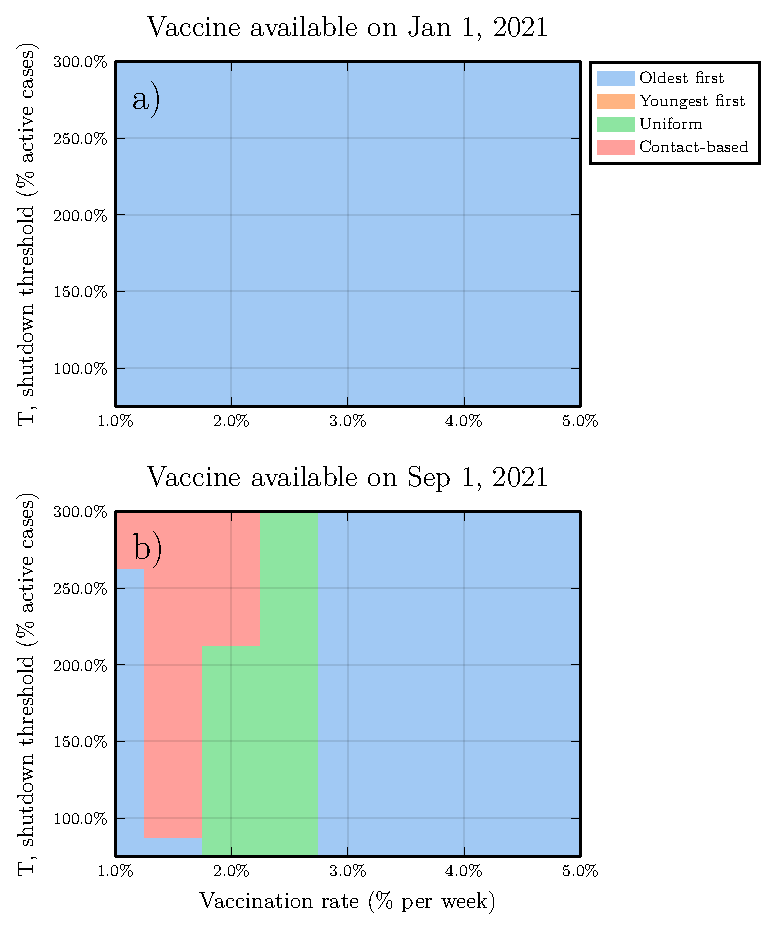
\includegraphics[width = 14 cm]{FigureS22.pdf}
\caption{\textbf{Sensitivity analysis for the scenario of one-fourth the baseline social learning rate from December 2020 onward.} Subpanels are parameter planes for January and September availability showing the vaccination strategy that reduces COVID-19 mortality the most as a function of $T$ and $\psi_0$.  Other parameter values as in Table S1.}
\label{plot_model}
\end{figure}

\clearpage 

\begin{figure}[H]
\centering
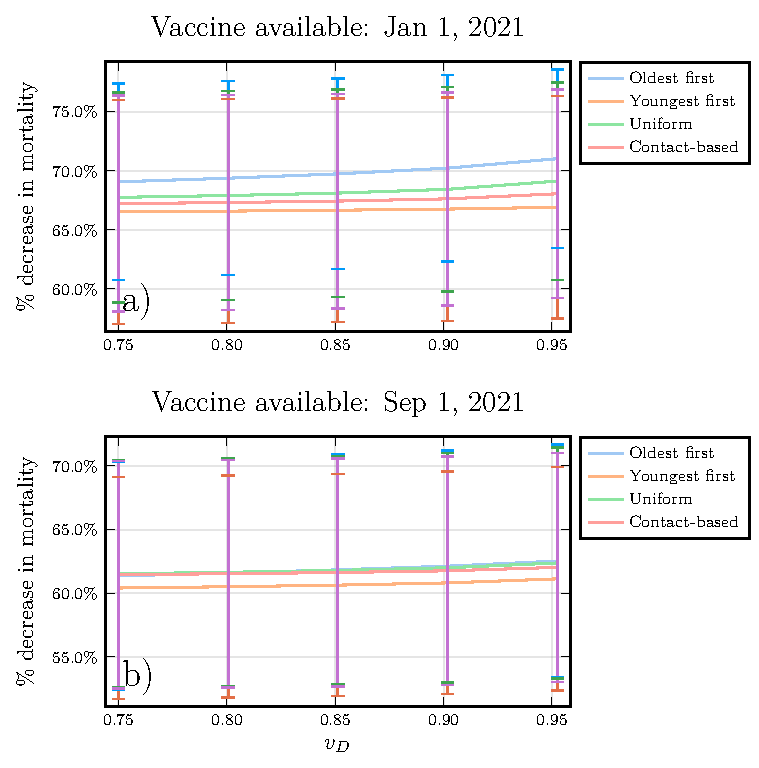
\includegraphics[width = 14 cm]{FigureS23.pdf}
\caption{\textbf{Sensitivity analysis for the scenario where efficacy against disease $v^D$ is not the same as efficacy against transmission $v^T$.} Subpanels show percentage reduction in mortality for the four stategies versus $v^D$ when $v^T=0.75$ but $v^D$ ranges from $0.75$ to $0.95$, for January and September availability.  Other parameter values as in Table S1.  Note that mortality in this plot is computed from March 15, 2020 to March 14, 2025.}
\label{plot_model}
\end{figure}

\clearpage 


\begin{figure}[H]
\centering
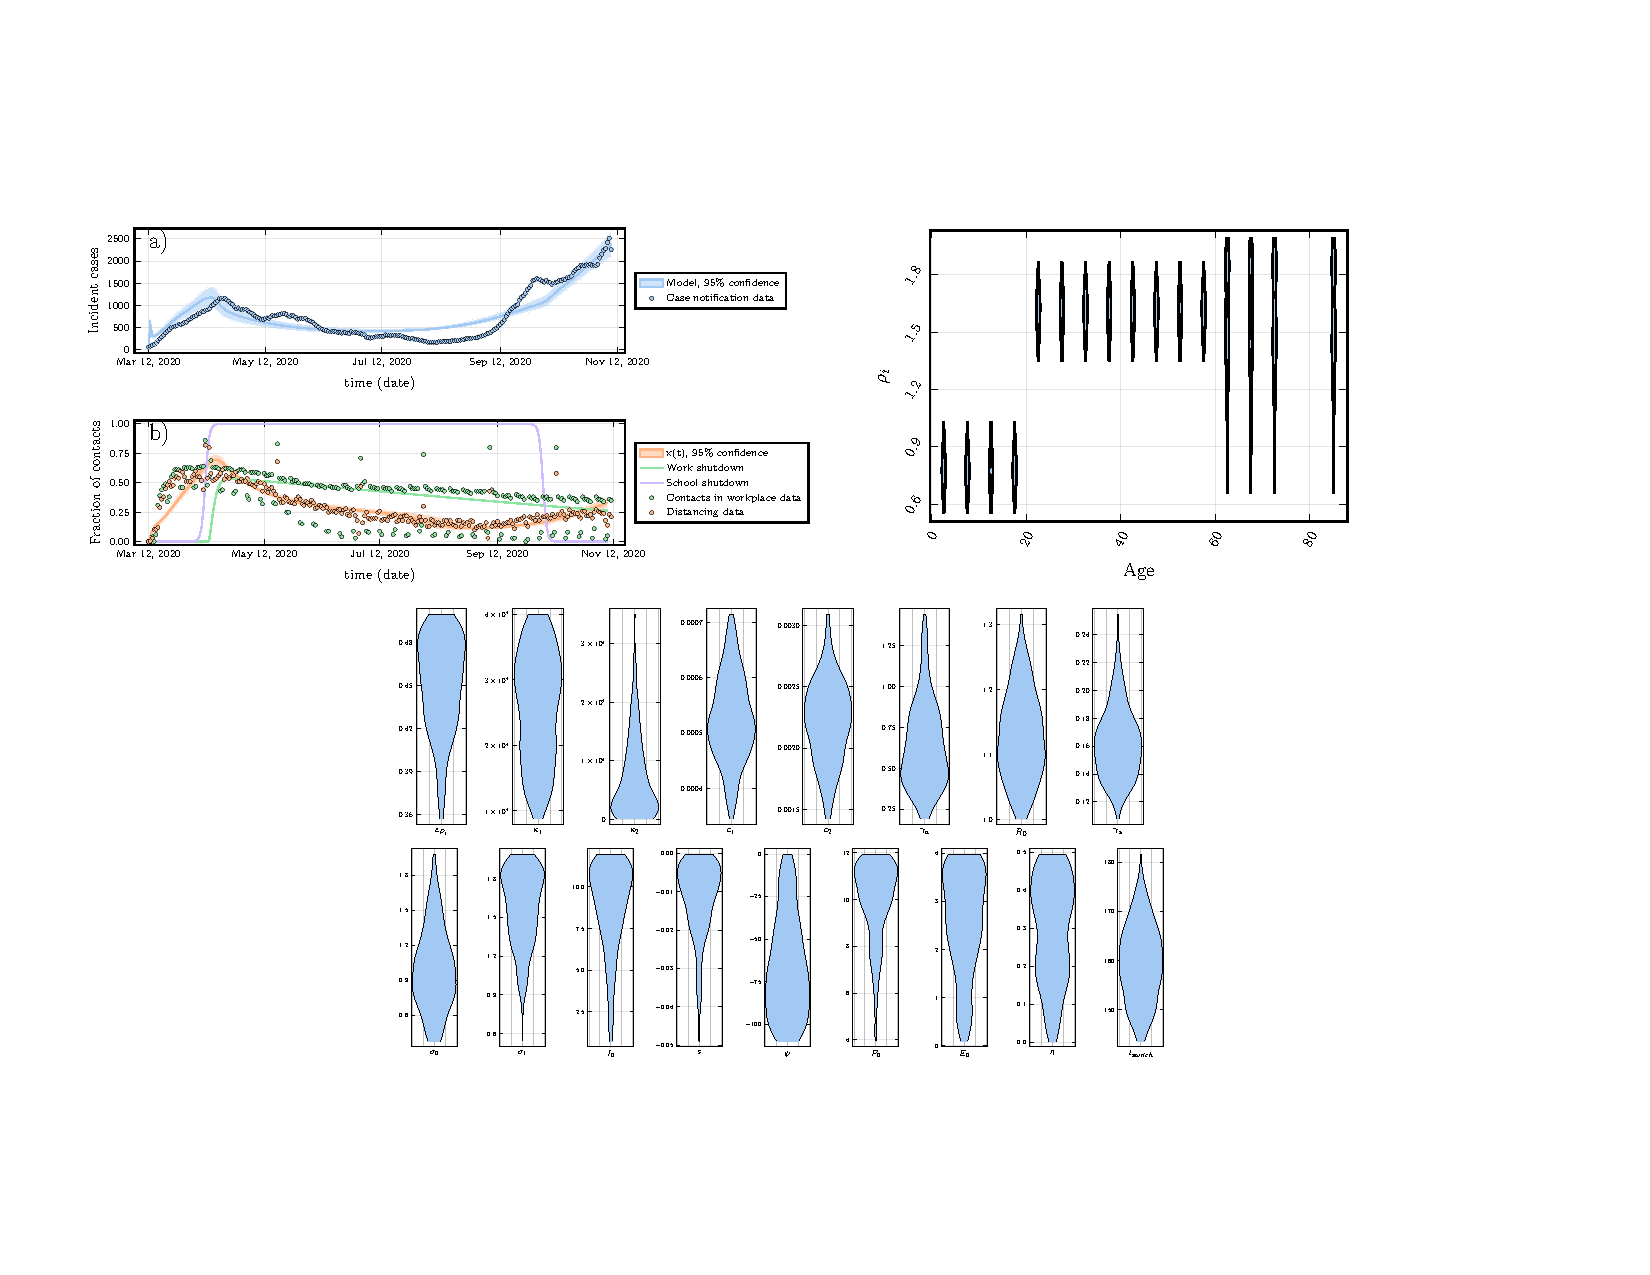
\includegraphics[width = 16 cm]{FigureS24.pdf}
\caption{\textbf{Posterior parameter distributions and model outputs for more stringent particle filtering criteria under Bayesian particle filtering algorithm.} Top left panel shows (a) COVID-19 case incidence by date of report in Ontario, 7-day running average (circles) and ascertained case incidence from best fitting models (lines). (b) Percentage change from baseline in time spent at retail and recreation destinations (orange circles) and at workplaces (green circles) from Google mobility data, and proportion of the population x adhering to NPIs (orange line) and workplace shutdown curve (green line) from fitted model.  Top right panel shows posterior parameter distribution for age-specific susceptibility modifier, $\rho_i$ . Bottom panel shows other posterior parameter distributions. Other parameter values as in Appendix, pp. 1-11.}
\label{plot_model}
\end{figure}

\begin{figure}[H]
\centering
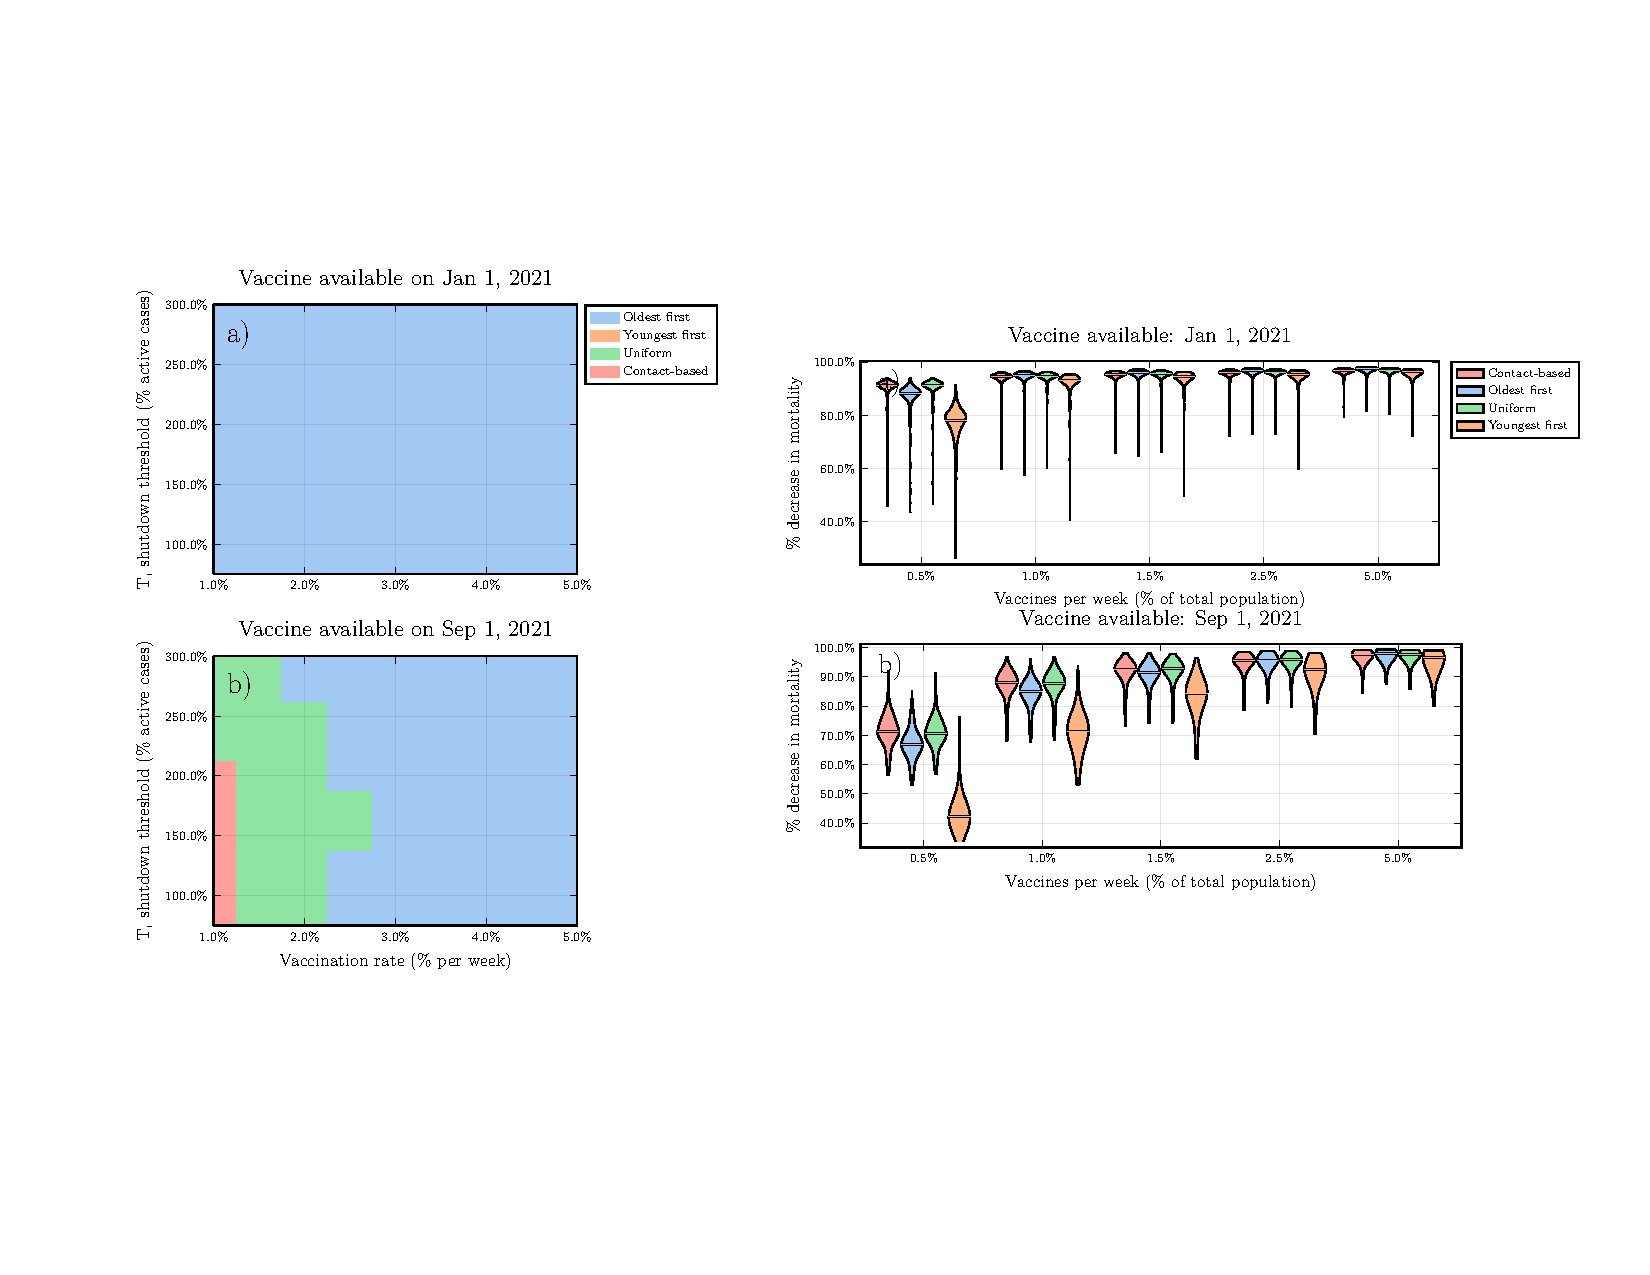
\includegraphics[width = 16 cm]{FigureS25.pdf}
\caption{\textbf{Sensitivity analysis for more stringent particle filtering criteria under Bayesian particle filtering algorithm.} Subpanels are parameter planes for January and September availability showing the vaccination strategy that reduces COVID-19 mortality the most as a function of $T$ and $\psi_0$ (left) and violin plots showing percentage reduction in mortality (right).  Horizontal lines represent median values of posterior model projections. Shutdown threshold T=200 \% and other parameter values in Appendix, pp. 1-11. Percentage reductions are relative to no vaccination. Projected number of deaths in the absence of vaccination was 72,000 (95\% credible interval: 40,000 to 122,000) from January 1, 2021 to March 14, 2025 for (a) and 60,000 (95\% credible interval: 31,000 to 108,000) from September 1, 2021 to March 14, 2025 for (b).  Ontario Population size: 14.6 million.}
\label{plot_model}
\end{figure}

\clearpage 

\begin{figure}[H]
\centering
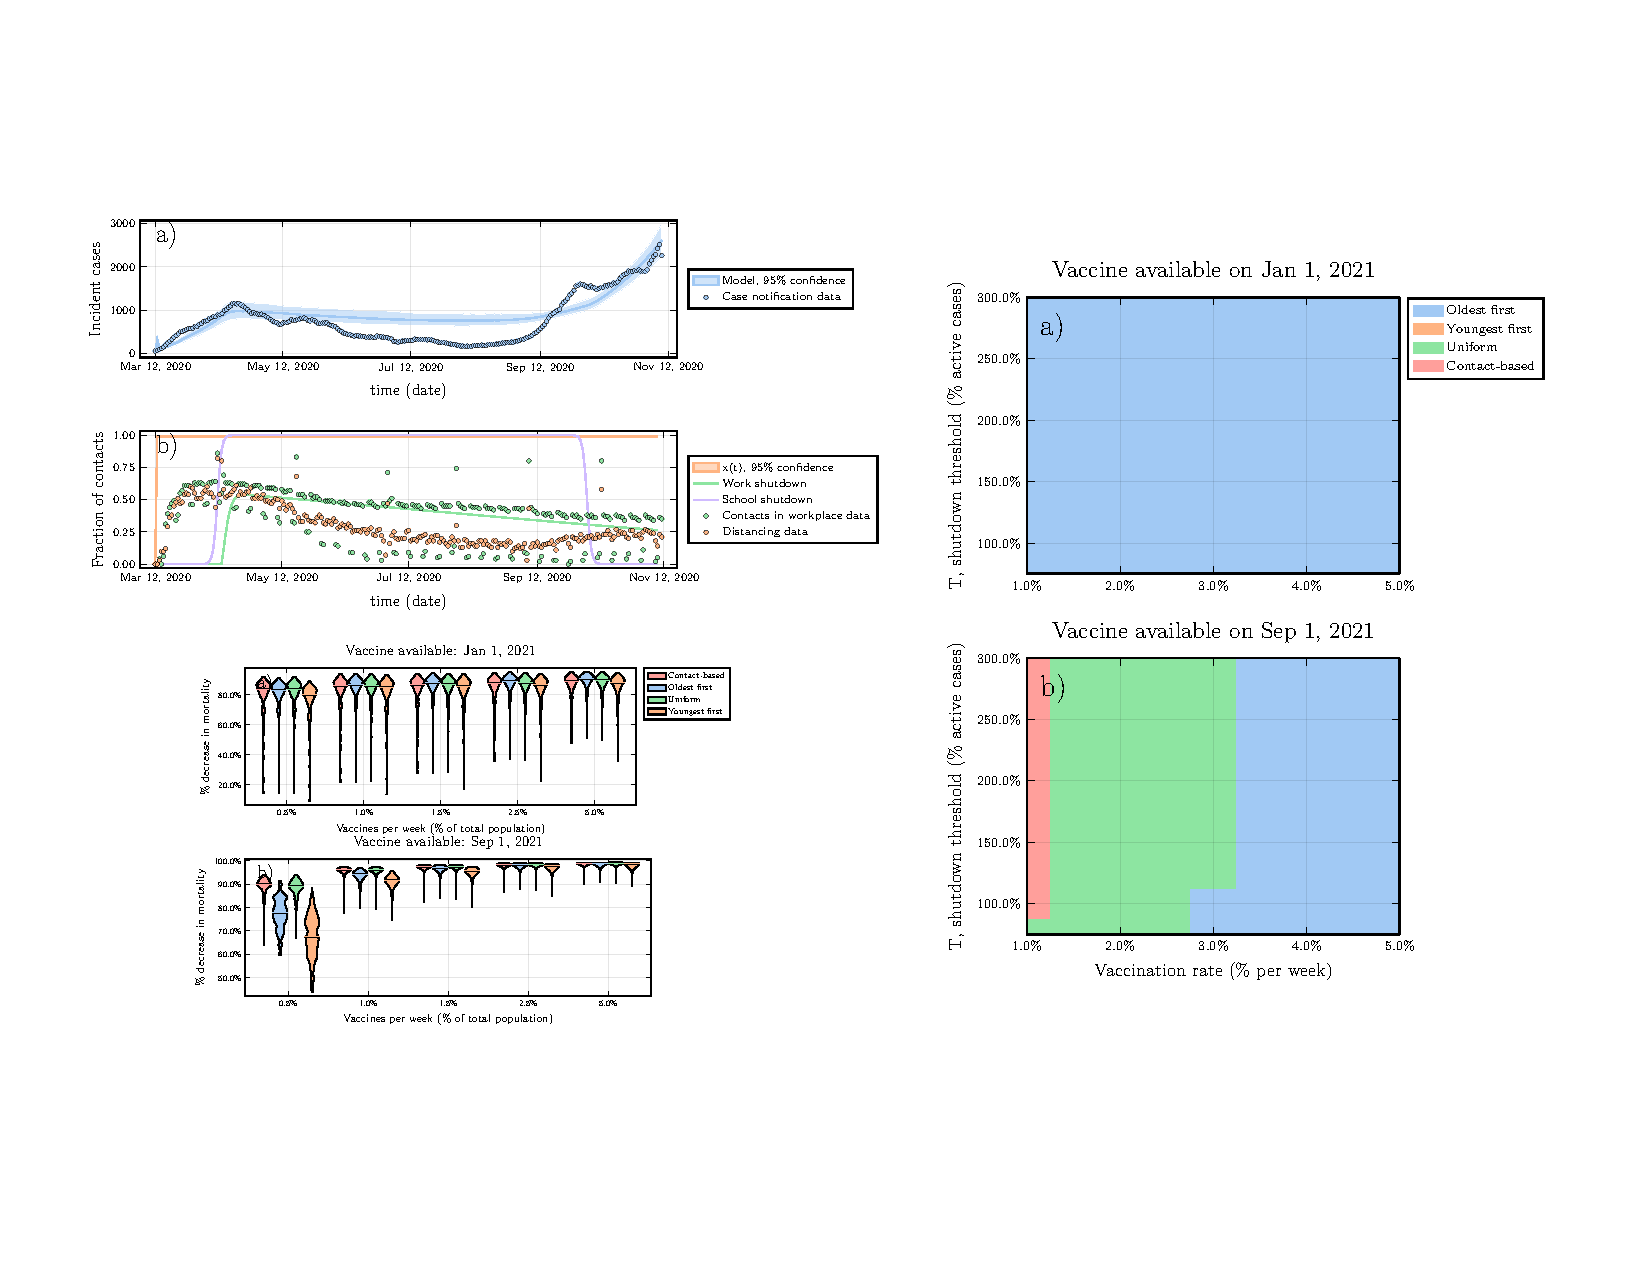
\includegraphics[width = 16 cm]{FigureS26.pdf}
\caption{\textbf{Model fit to data and baseline projections of mortality reductions under the four vaccine strategies, when behaviour is held constant over time.} Top left: a) COVID-19 case incidence by date of report in Ontario, 7-day running average (circles) and ascertained case incidence from best fitting models (lines). (b) Percentage change from baseline in time spent at retail and recreation destinations (orange circles) and at workplaces (green circles) from Google mobility data, and proportion of the population x adhering to NPIs (orange line) and workplace shutdown curve (green line) from fitted model. Bottom left: Violin plots of the percent reduction in mortality under the four vaccine strategies, relative to no vaccination, as a function of the vaccination rate ψ0, for (a) January and (b) September 2021 availability. Horizontal lines represent median values of posterior model projections. Shutdown threshold T=200\%. Percentage reductions are relative to no vaccination. Projected number of deaths in the absence of vaccination was 72,000 (95\% credible interval: 40,000 to 122,000) from January 1, 2021 to March 14, 2025 for (a) and 60,000 (95\% credible interval: 31,000 to 108,000) from September 1, 2021 to March 14, 2025 for (b).  Ontario Population size: 14.6 million.  Right:  Each parameter combination on the plane is colour coded according to which of the four strategies prevented the most deaths, on average across all model realizations, for (a) January and (b) September 2021 availability. Other parameter values in Appendix, pp. 1-11.}
\label{plot_model}
\end{figure}

\clearpage 

\begin{figure}[H]
\centering
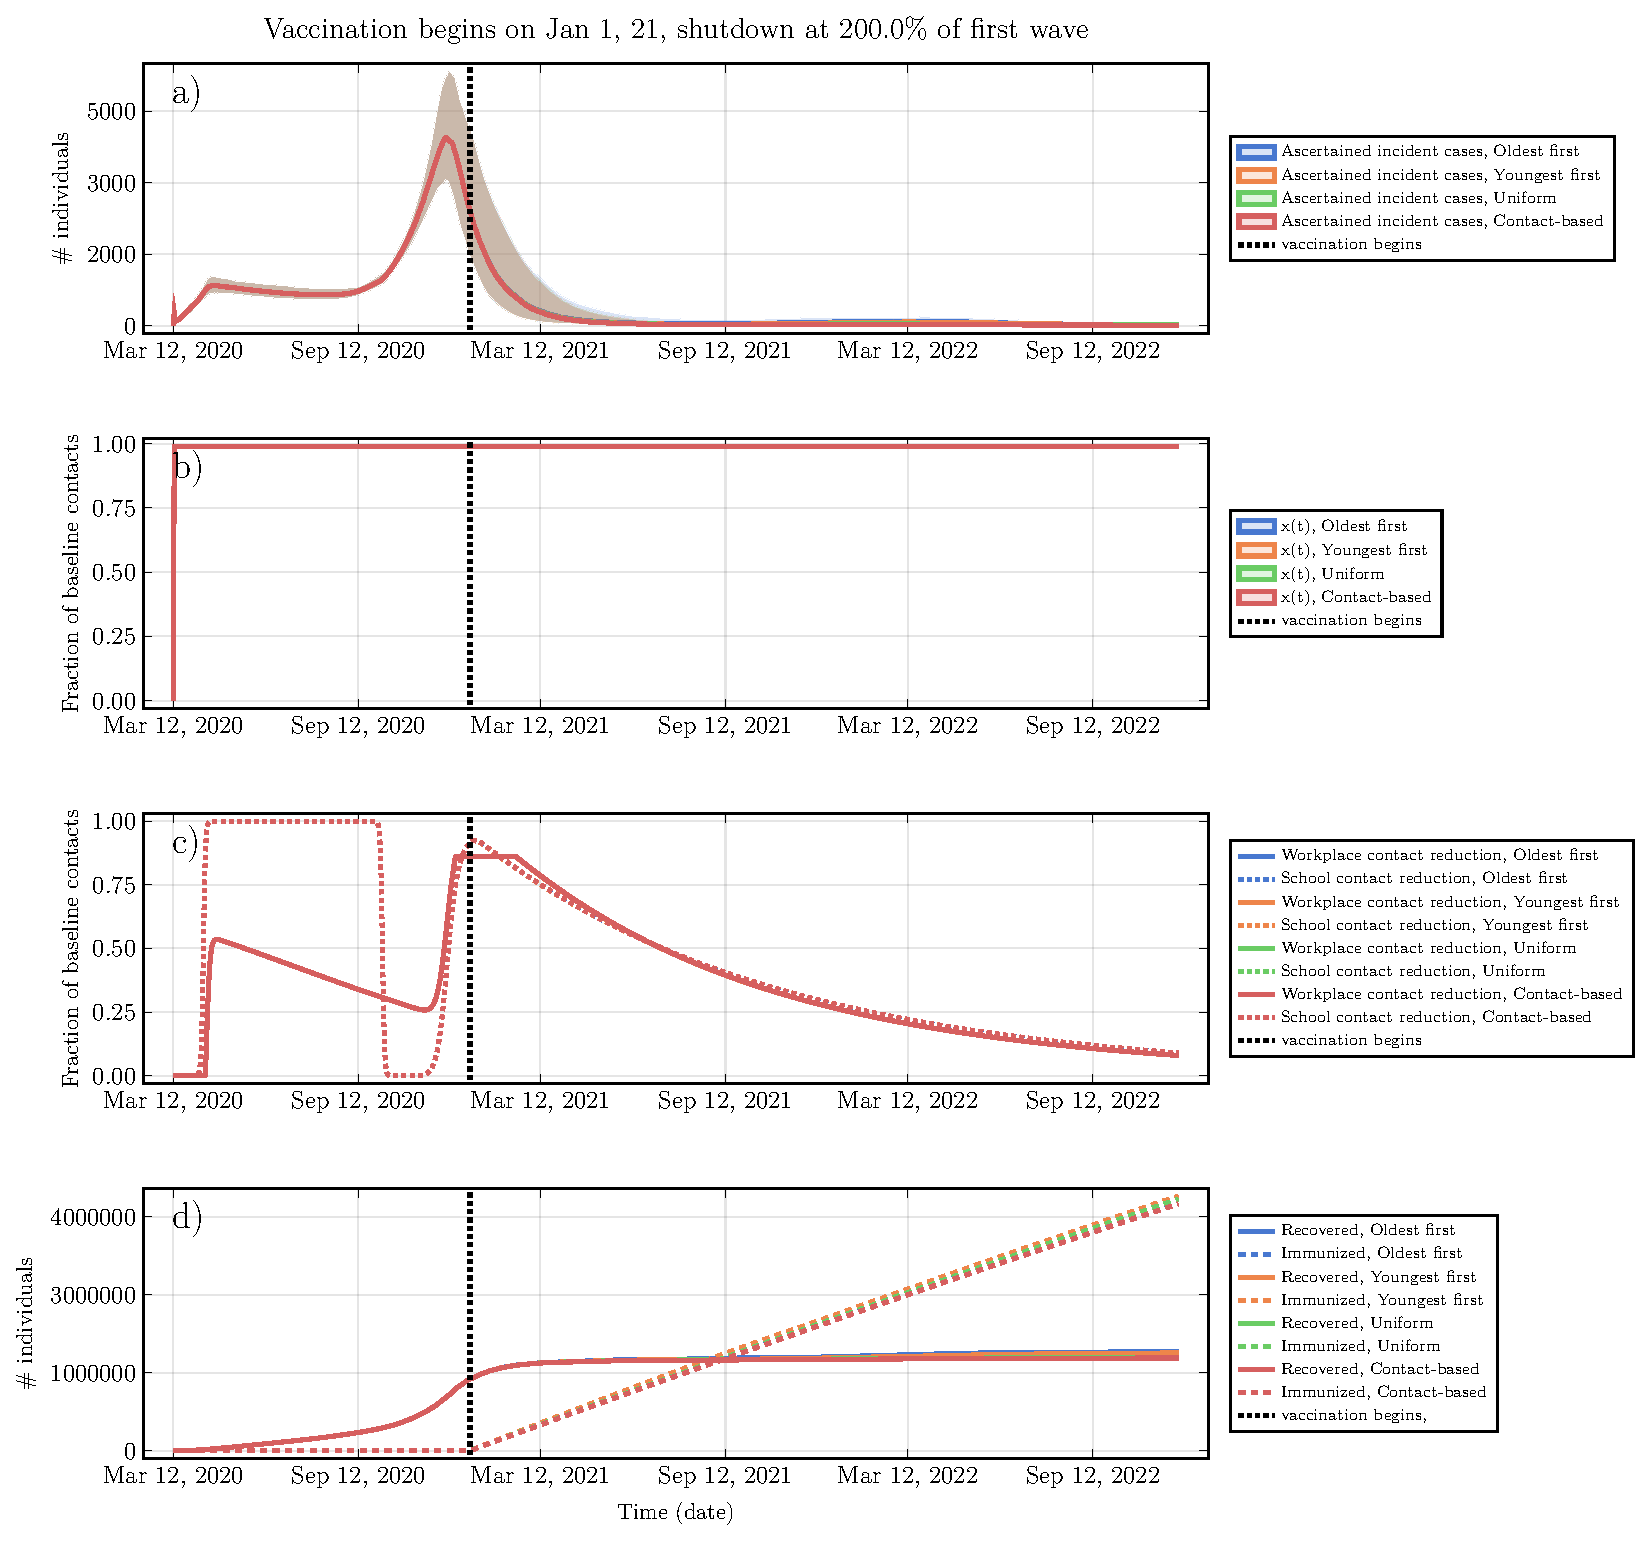
\includegraphics[width = 16 cm]{FigureS27.pdf}
\caption{\textbf{Epidemic dynamics and social dynamics for both NPI adherence and vaccinating behaviour, when behaviour is held constant over time.} (a) Ascertained incident COVID-19 cases, (b) proportion $x$ of the population practicing NPIs, (c) Intensity of school and workplace closure, (d) percentage of population with natural or vaccine-derived immunity versus time. $T=200 \%$, $\psi_0=0.5 \%$ per week, vaccine available in January 2021. Other parameters are in Table \ref{tab:params}.}
\label{plot_model}
\end{figure}

\clearpage 

%\begin{figure}[H]
%\centering
%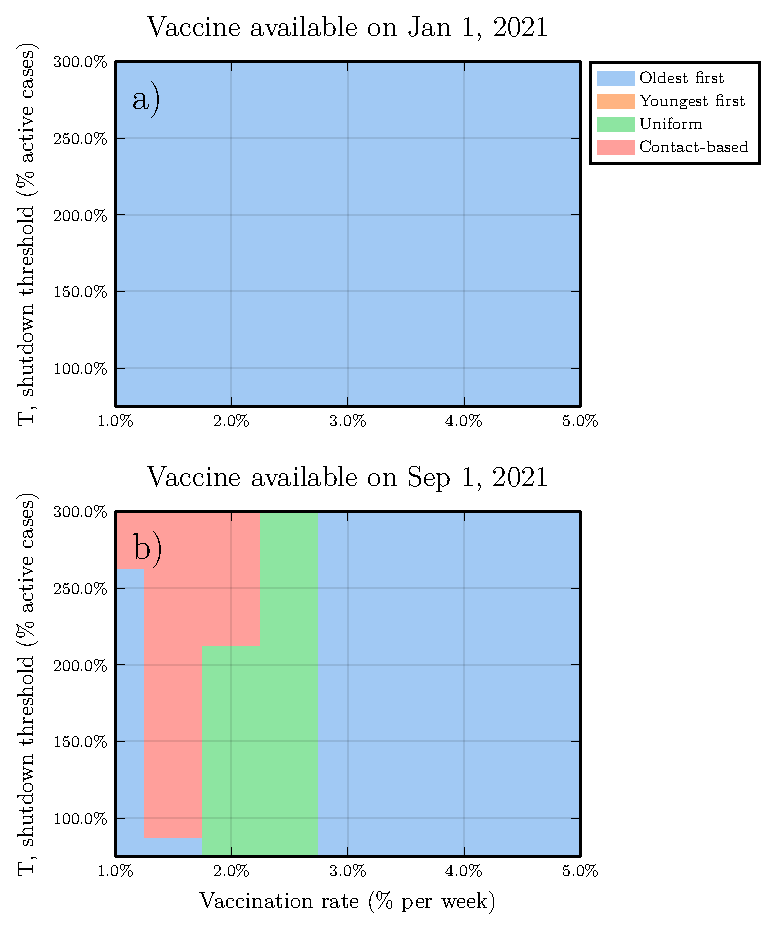
\includegraphics[width = 18 cm]{FigureS22.pdf}
%\caption{\textbf{Sensitivity analysis for the scenario where behaviour is constant over time.} Subpanels are  (left) parameter planes for March and September availability showing the vaccination strategy that prevents the most COVID-19 deaths as a function of $T$ and $\psi_0$, (top right) percentage reductions in mortality, and (bottom right) the corresponding posterior parameter distributions for the refitted parameters. Other parameter values are as in Table S1.}
%\label{plot_model}
%\end{figure}

%\clearpage 

%\begin{figure}[H]
%\centering
%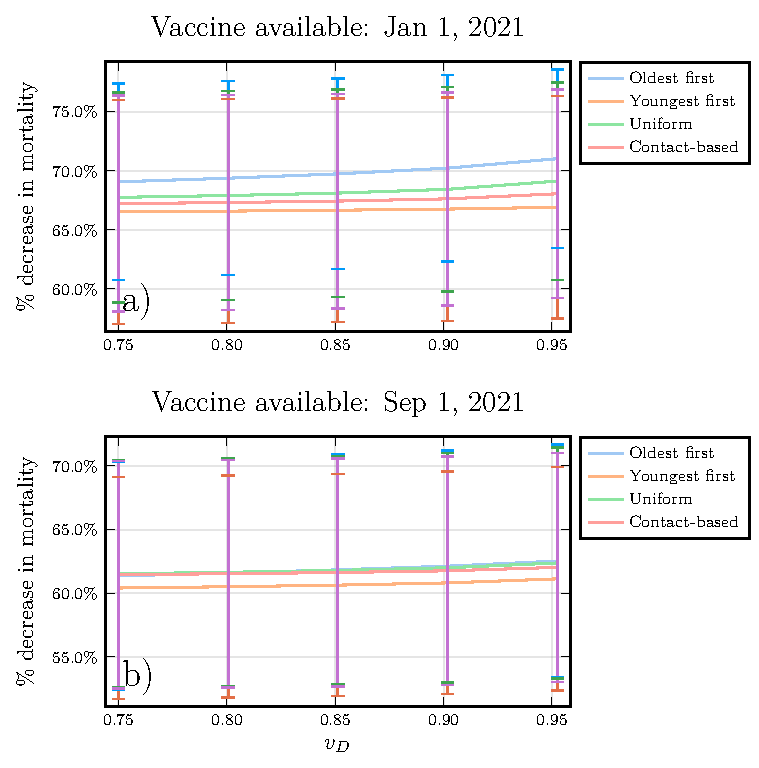
\includegraphics[width = 18 cm]{FigureS23.pdf}
%\caption{\textbf{Sensitivity analysis for the scenario where there is no seasonality in transmission.} Subpanels are  (left) parameter planes for March and September availability showing the vaccination strategy that prevents the most COVID-19 deaths as a function of $T$ and $\psi_0$, (top right) percentage reductions in mortality, and (bottom right) the corresponding posterior parameter distributions for the refitted parameters. Other parameter values are as in Table S1.}
%\label{plot_model}
%\end{figure}


%%%%%%%%%%%%%%%%%%%%%%%%%%%%%%%%%%%%%%%%%%%%


%\begin{figure}[H]
%\centering
%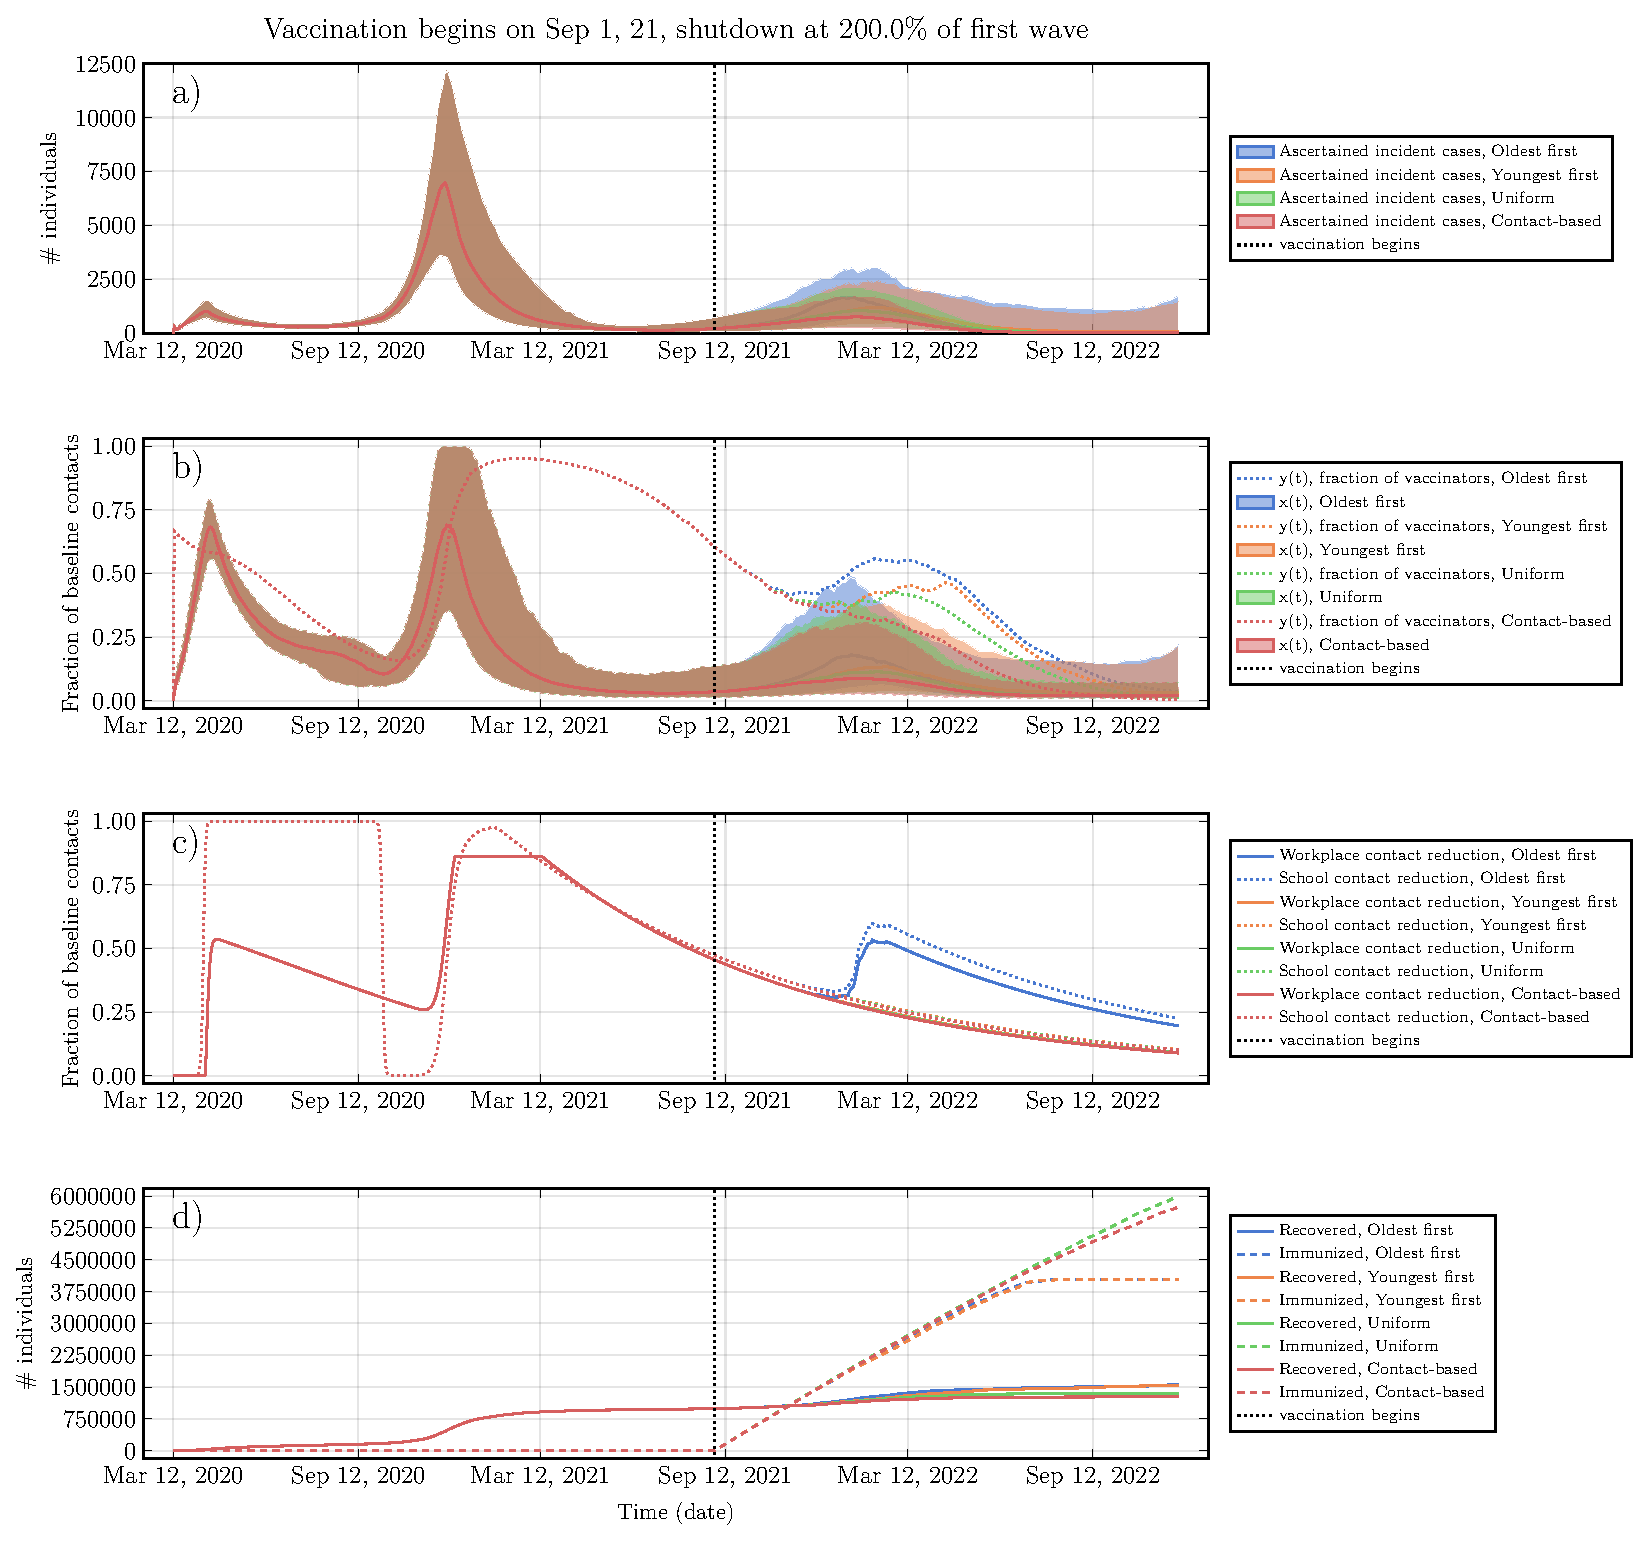
\includegraphics[width = 18 cm]{FigureS17.pdf}
%\caption{\textbf{Sensitivity analysis for the scenario of $50 \%$ heightened social learning rate from December 2020 onward.} Subpanels are parameter planes for March and September availability showing the vaccination strategy that reduces COVID-19 mortality the most as a function of $T$ and $\psi_0$ (left) and the corresponding posterior parameter distributions for the refitted parameters (right).  Other parameter values as in Table S1.}
%\label{plot_model}
%\end{figure}

%\clearpage 

%\begin{figure}[H]
%\centering
%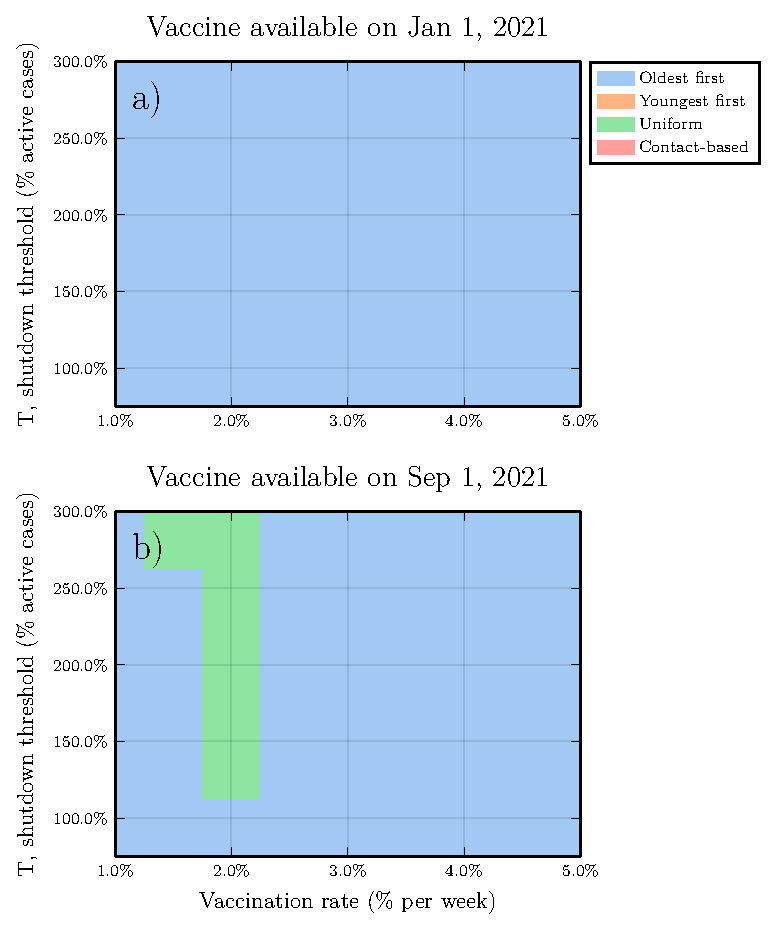
\includegraphics[width = 18 cm]{FigureS18.pdf}
%\caption{\textbf{Sensitivity analysis for the scenario of $50 \%$ reduced social learning rate from December 2020 onward.} Subpanels are parameter planes for March and September availability showing the vaccination strategy that reduces COVID-19 mortality the most as a function of $T$ and $\psi_0$ (left) and the corresponding posterior parameter distributions for the refitted parameters (right).  Other parameter values as in Table S1.}
%\label{plot_model}
%\end{figure}

%\clearpage 


\section*{Supplementary Appendix References}
\bibliography{pnas-sample}

\end{document}
